\chapter{Beam tests}\label{chap::6}

\vfill

\minitoc

\newpage

\glsresetall
\glsunset{clarys} 


As described in chapter~\ref{chap::3}, the components of the \gls{clarys} gamma cameras are at the final characterization phase, and the efforts of the collaboration are presently mainly focused on the optimization of the acquisition chain, including the electronics boards, the \gls{utca} acquisition system and the associated acquisition, monitoring and slow control software. These tasks foresee several measurements campaigns, and three of them have been performed between the end of 2017 and the date of writing (September 2018), and are presented in this chapter. 
All the presented beam tests have been carried out at the \gls{cal} with a 65~MeV proton beam. 

The Nice hadrontherapy platform was the first site in France starting to treat patients in June 1991 with the MEDYCIC cyclotron proton beams. The cyclotron was designed to support regular neutron and proton therapy programs, as well as for the production of $^{18}$F for \gls{pet} applications~\parencite{Mandrillon1989, Mandrillon1992}. The accelerator is a fixed frequency 25~MHz isochronous cyclotron with a peak voltage of 50kV. Negative hydrogen ions are produced by an external source, axially injected and accelerated to 65~MeV. The extraction is performed by a 60$\times$10$^{-6}$ g/cm$^2$ carbon stripping foil and the exiting protons are transported down the beam line to the treatment room~\parencite{Herault2005}, or to the research nozzle used for the presented beam tests. The layout of the MEDICYC facility is shown in \figurename~\ref{chap6::fig::MEDICYC_layout}. The details of the center layout are sketched in \figurename~\ref{chap6::fig::MEDICYC_layoutDetails}, showing the cyclotron , the beam line, the proton therapy treatment room, and the research-dedicated line. The beam is bent by 90\textdegree ~to be sent to the treatment room, while it is extracted without deflection for research purpose.

 \begin{figure}[!htbp]
\centering
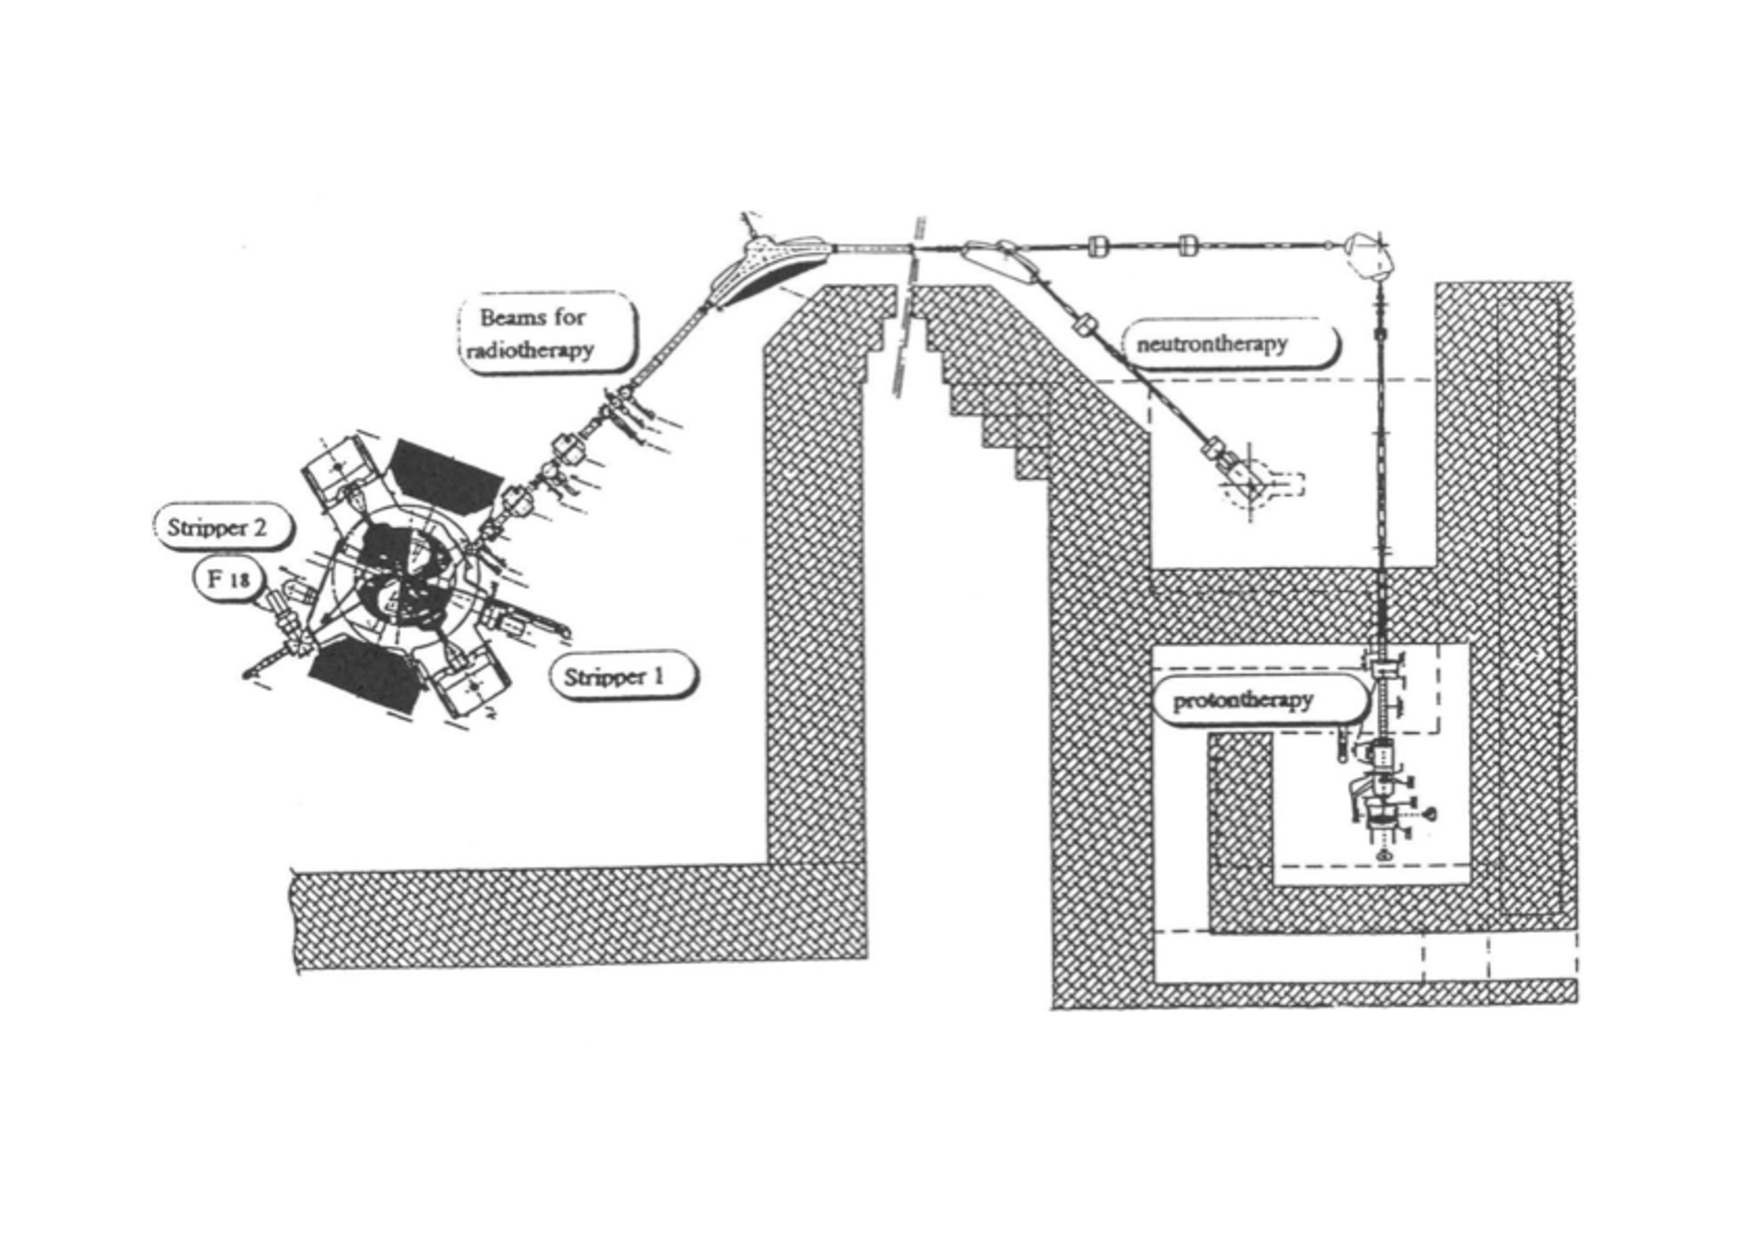
\includegraphics[width=0.6\textwidth]{03_GraphicFiles/chapter6_BeamTests/MEDiCYC.pdf}
\caption{Layout of the Nice MEDICYC facility. In~\cite{Mandrillon1992}.}
\label{chap6::fig::MEDICYC_layout}
\end{figure}

 \begin{figure}[!htbp]
\centering
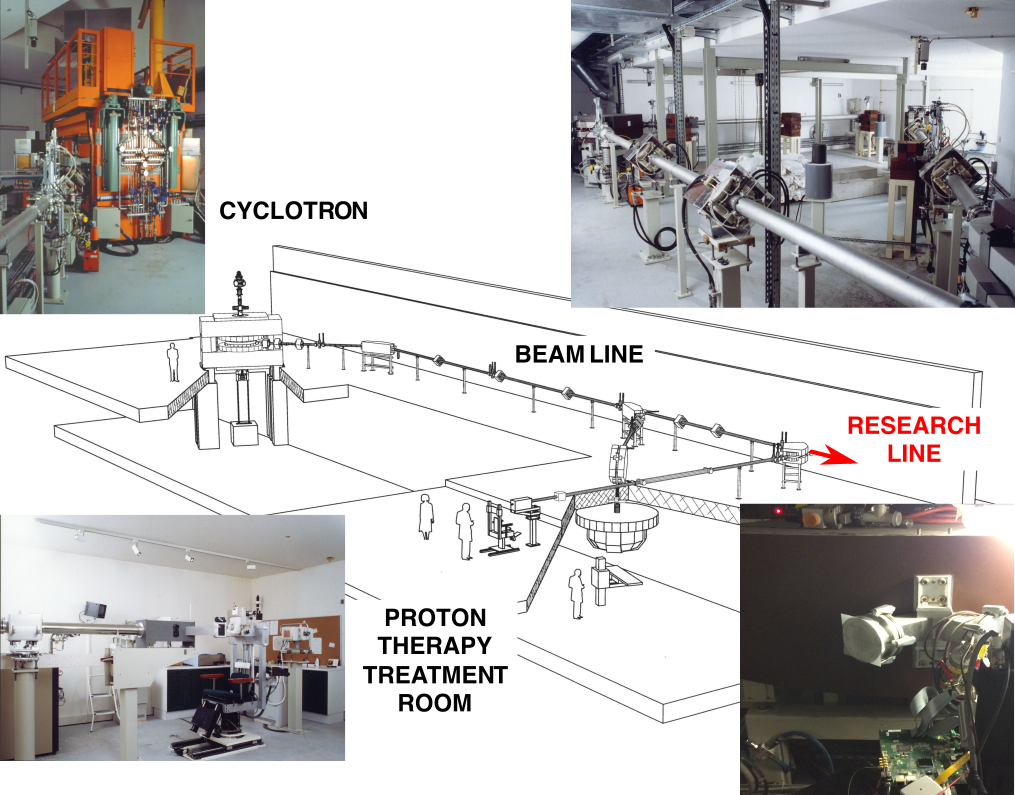
\includegraphics[width=0.7\textwidth]{03_GraphicFiles/chapter6_BeamTests/MEDICYC_scheme.png}
\caption{Layout of the Nice MEDICYC facility with pictures of the components: cyclotron, beam line, and treatment room. The beam nozzle dedicated to research activities is shown by the red arrow (also showing the beam direction) and shown in the picture in the bottom right corner of the scheme.}
\label{chap6::fig::MEDICYC_layoutDetails}
\end{figure}

The \gls{cal} is at present equipped with a Proteus One \gls{iba} treatment facility, with an S2C2 cyclotron~\parencite{Pearson2013}, which is has been finalized in June 2016. The MEDICYC low energy treatment line is dedicated to ocular tumors, while the new high-energy facility allows to treat all other kinds of tumors.

We started from testing the hodoscope acquisition chain in December 2017. As a first minimal approach, the 32$\times$32 fiber hodoscope has been used, given the fact that it can be read out by a single \gls{fe} board, and no synchronization capabilities are required in the \gls{fe} board firmware. The December test allowed to highlight the main limitations affecting the \gls{fe} board, as well as the software governing the \gls{utca} acquisition system.
In the following months, an extensive revision work has been dedicated to the hodoscope \gls{fe} board and to the \gls{utca} firmware. The acquisition software has been also optimized for higher data throughput.  
A new beam test dedicated to the 32$\times$32 fiber hodoscope has been carried out in May 2018, and it is detailed in section~\ref{chap6::sec::may2018}. This test allowed to have a first characterization of the hodoscope with the final acquisition chain on beam, to evaluate the needed improvements and plan the test of first multi-collimated camera configuration. In the following months, indeed, the attention has been focused on the \gls{bgo} absorber blocks, and the read-out through \gls{asm} boards and  \gls{utca} system has been developed at the \gls{ipnl}. A minimal collimated camera setup, including the 32$\times$32 fiber hodoscope (read-out with a single hodoscope \gls{fe} board) and 6 \gls{bgo} blocks (read-out with a single \gls{asm} board) has been tested on beam in the second half of September 2018. The test details are given in section~\ref{chap6::sec::september2018}. 
 
\section{Hodoscope: May 2018}\label{chap6::sec::may2018}
After the improvements implemented on the hodoscope \gls{fe} board and \gls{utca} firmware which followed the first preliminary test in December 2017, the 32$\times$32 fiber hodoscope has been tested with the same configuration in May 2018. The acquisition logic allows to operate the hodoscope in triggered and stand-alone mode: in the first case, the trigger signal is given by the absorber in the collimated camera setup, or by the coincidence between absorber and scatterer in the Compton camera setup. For this test, an external trigger has been provided thanks to two 5$\times$5~cm$^2$ plastic scintillators, read-out by a \gls{pm}, placed on beam upstream and downstream with respect to the hodoscope. The plastic scintillators have been aligned to the hodoscope and one to the other, in order to fully cover the hodoscope active area of 3.2$\times$3.2~cm$^2$. The hodoscope was placed at a distance of 15~cm from the beam nozzle, the plastic scintillator upstream was approximately at 10~cm, the one downstream at 19~cm. A schematic view of the test setup is given in \figurename~\ref{chap6::fig::May_HodoDAQscheme}, and two pictures of the system are shown in \figurename~\ref{chap6::fig::May_HodoSetup}. 


\begin{figure}[!htbp]
\centering
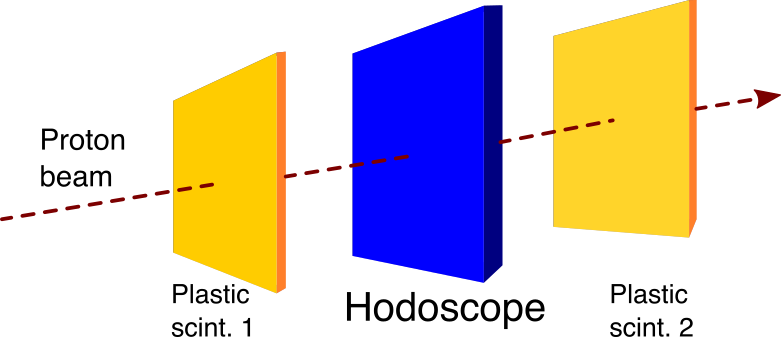
\includegraphics[width=0.7\textwidth]{03_GraphicFiles/chapter6_BeamTests/Nice_May2018/scheme.png}
\caption{Schematic view of the hodoscope and plastic scintillator setup along the beam line.}
\label{chap6::fig::May_HodoDAQscheme}
\end{figure}

\begin{figure}[!htbp]
\begin{subfigure}[t]{.5\textwidth}
\centering
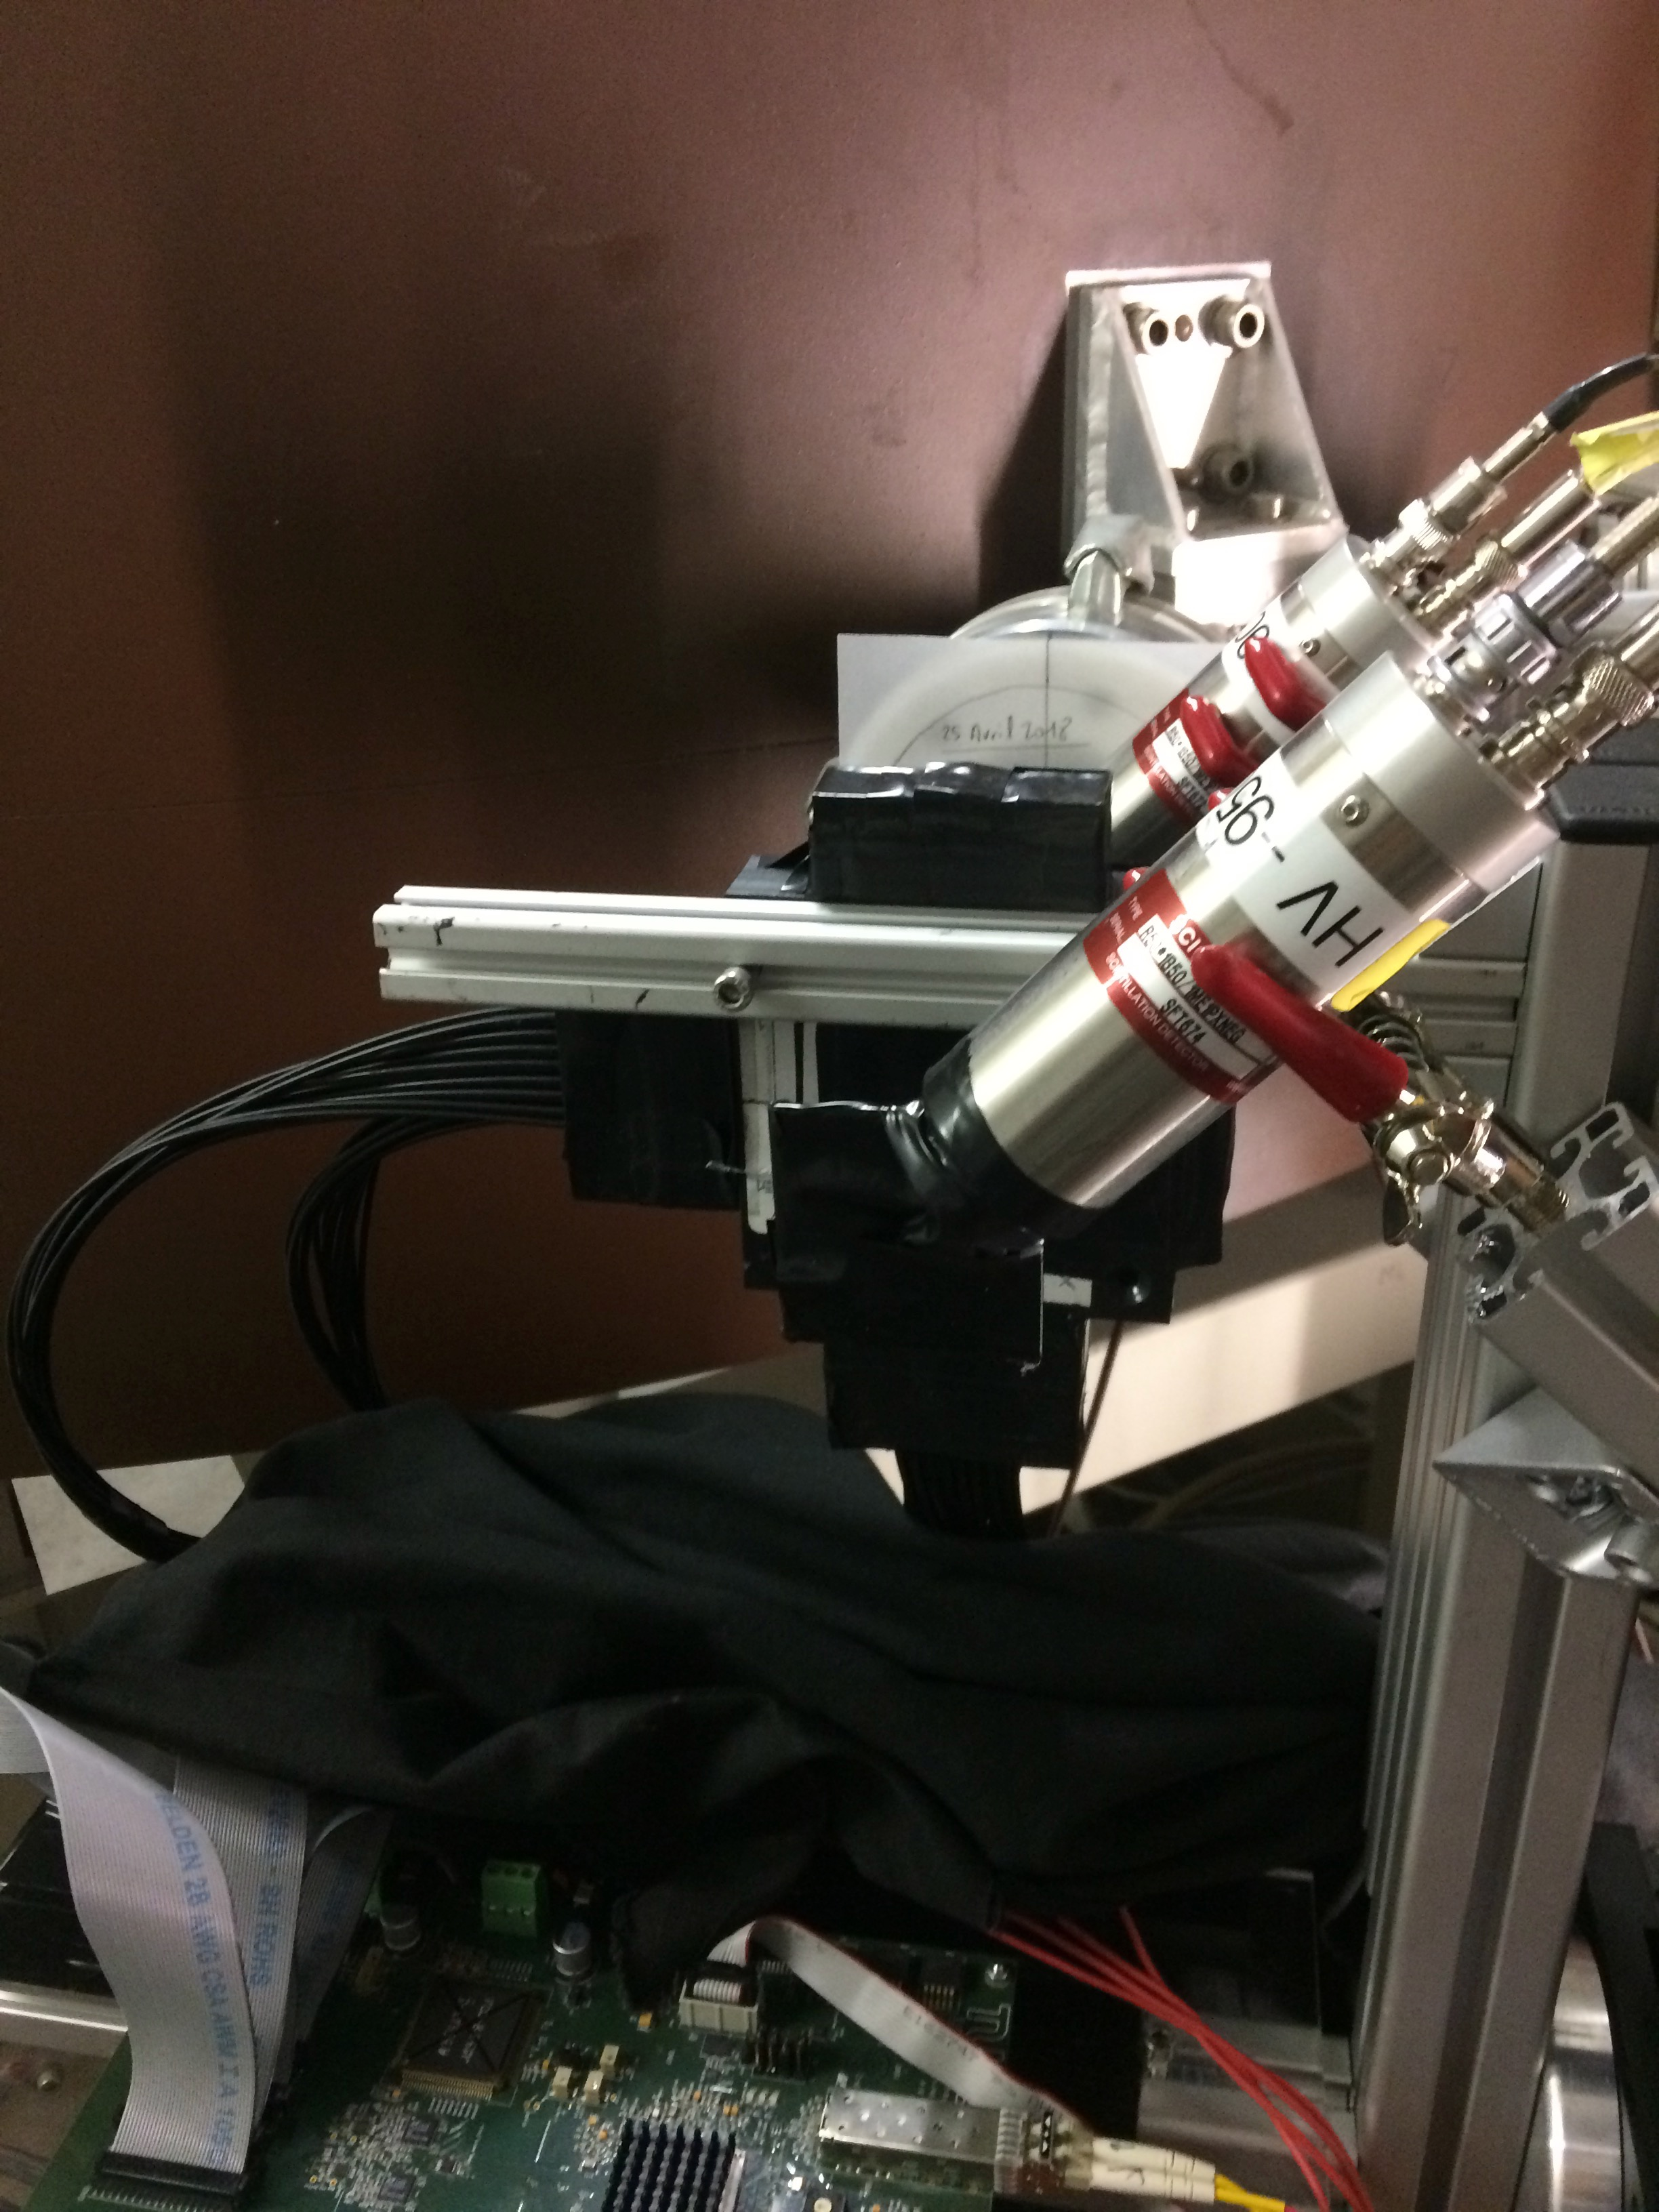
\includegraphics[width=0.9\textwidth]{03_GraphicFiles/chapter6_BeamTests/Nice_May2018/IMG_5181.jpg}
\caption{Picture of the beam test setup from downstream the beam nozzle. The two 5~cm side plastic scintillators are st one upstream and one down stream with respect to the hodoscope. All the system is mounted on a custom support.}
\label{chap6::fig::May_HodoSetupPicture2}
\end{subfigure}
\begin{subfigure}[t]{.5\textwidth}
\centering
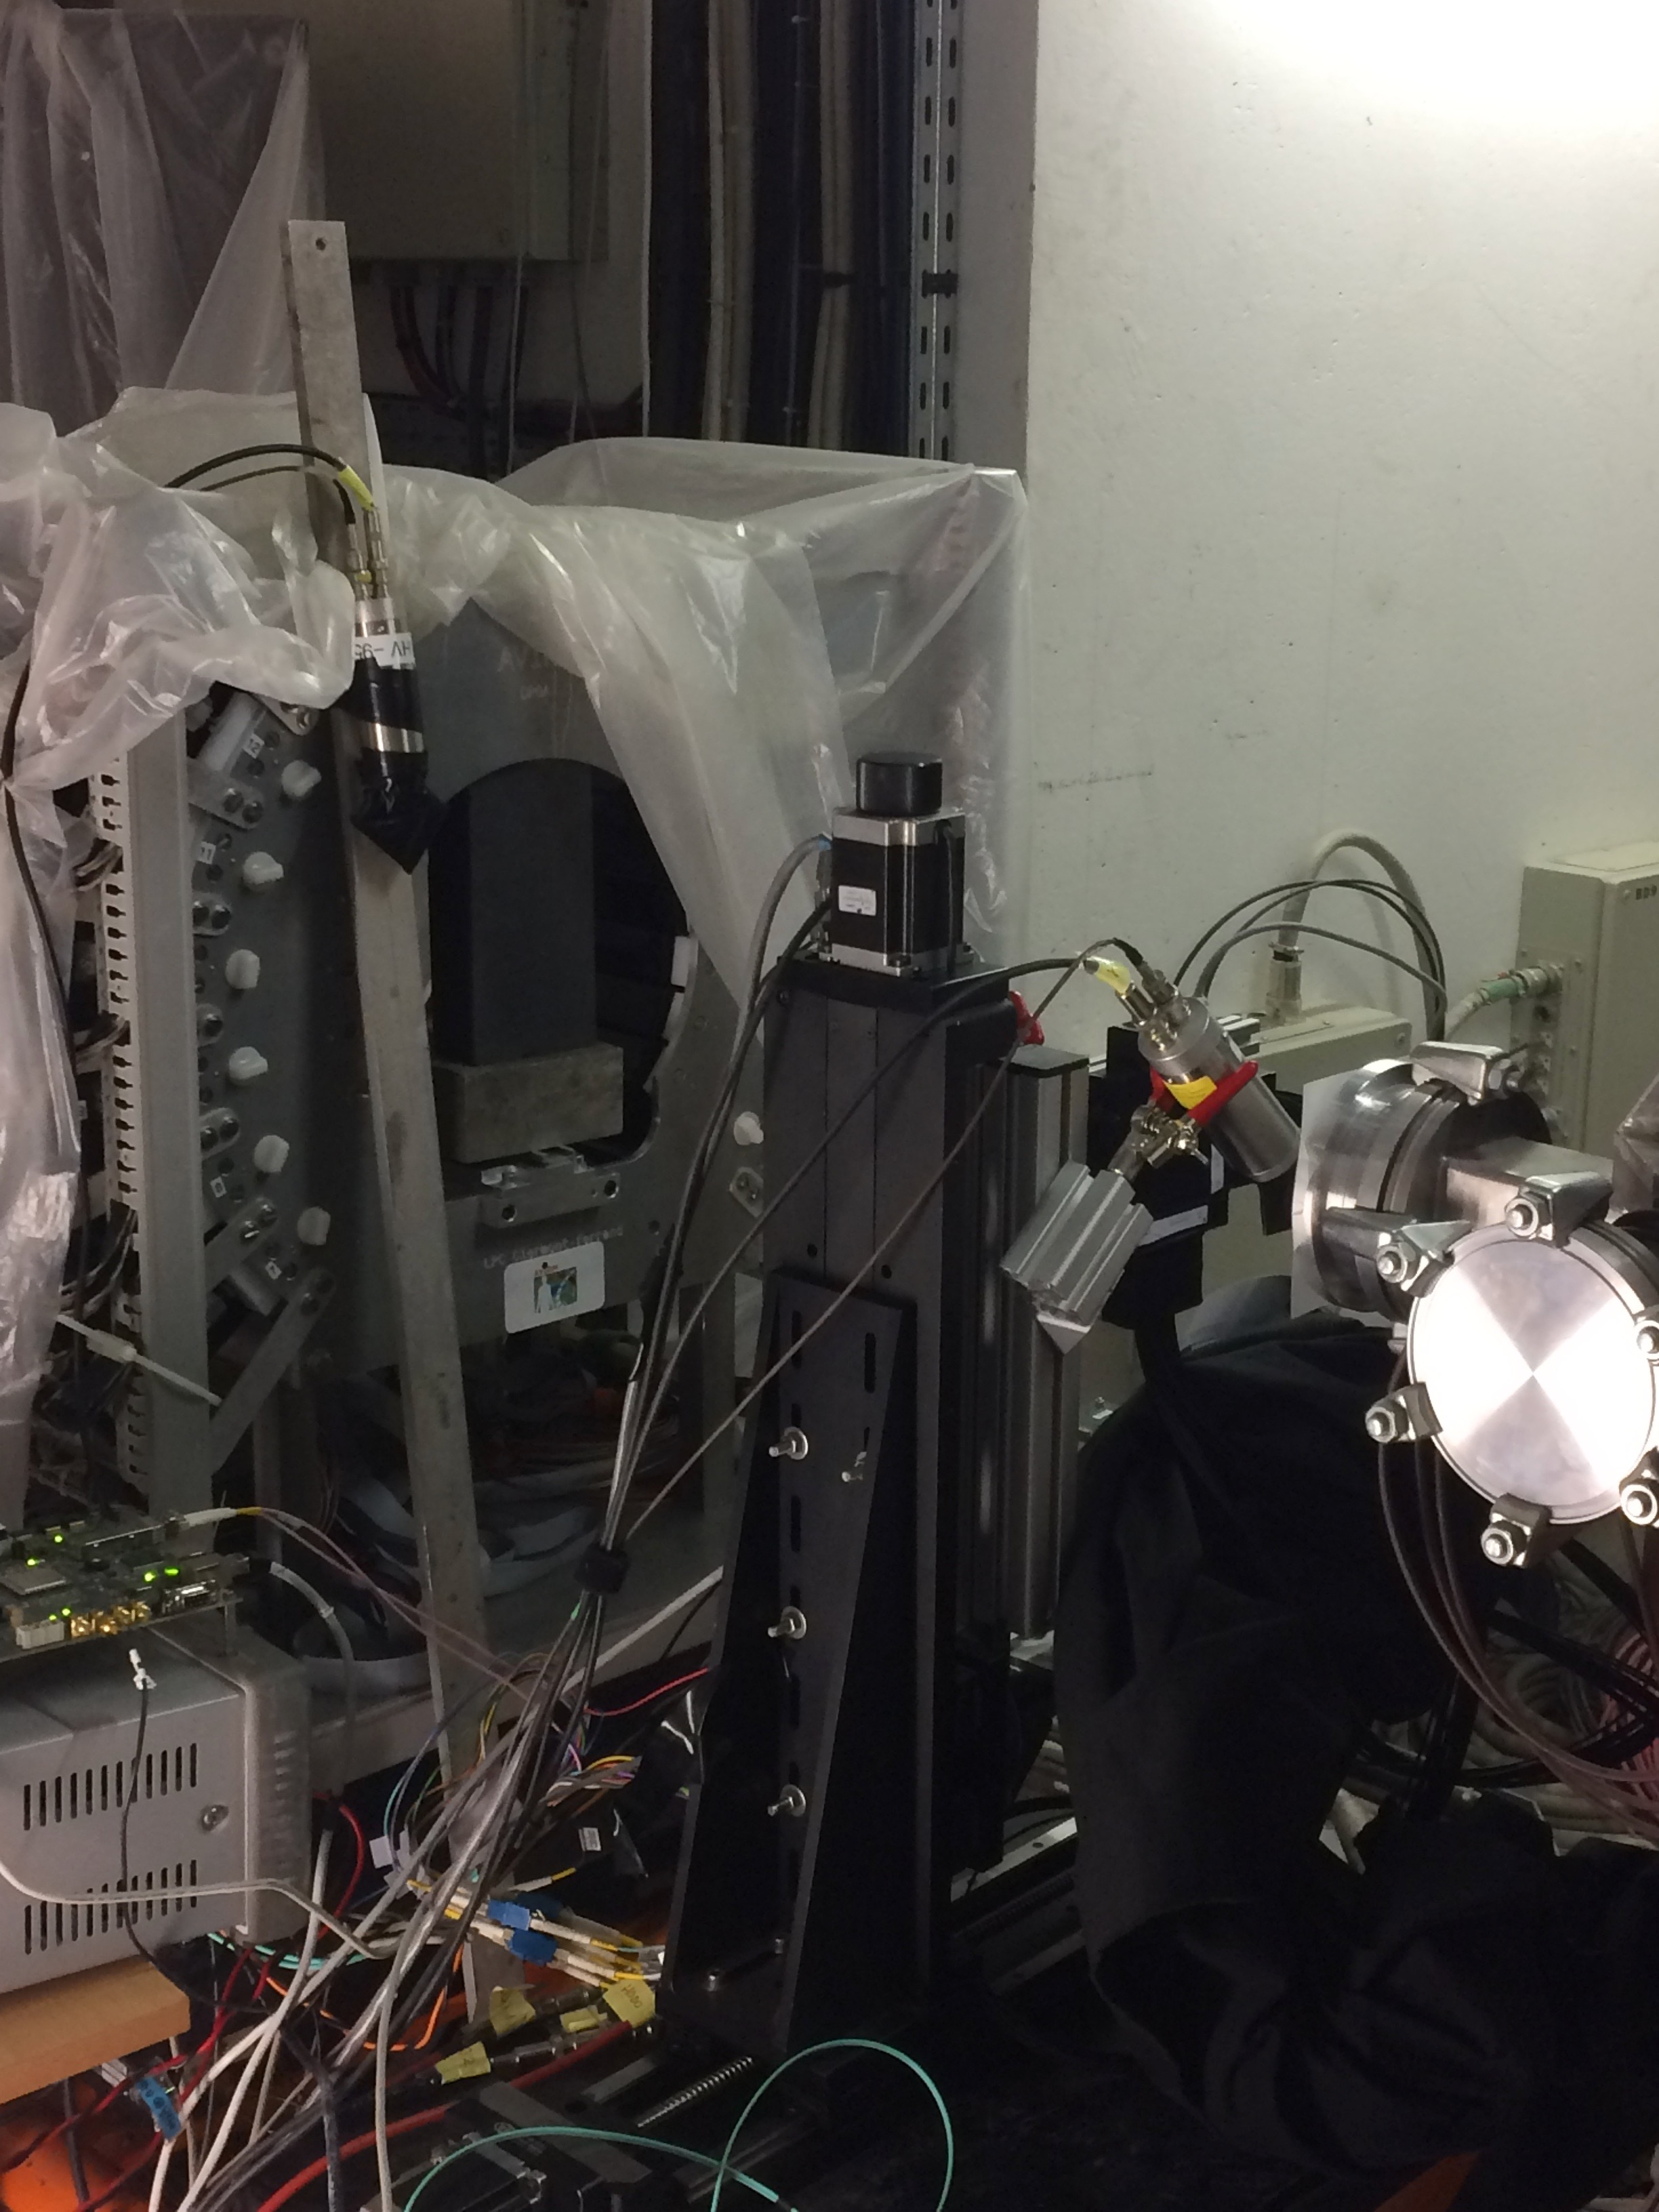
\includegraphics[width=0.9\textwidth]{03_GraphicFiles/chapter6_BeamTests/Nice_May2018/IMG_5186.jpg}	
\caption{Picture of the complete beam test setup. Hodoscope and trigger scintillators are fixed to a two-dimensional moving table and set at approximately 15~cm from the nozzle (from the nozzle to the hodoscope center). A third plastic scintillator is fixed outside the beam line (top left corner) to provide intensity monitoring at the high rates not supported by the scintillators on beam.}
\label{chap6::fig::May_HodoSetupPicture}
\end{subfigure}
\caption{Pictures of the hodoscope test setup.}
\label{chap6::fig::May_HodoSetup}
\end{figure}

The hodoscope and the two plastic scintillators have been mounted on the two-dimensional moving table described in chapter~\ref{chap::3}, to adjust the setup position with respect to the beam nozzle. 
The analogical output of the two plastic scintillator was treated with standard \gls{nim} modules: each single signal was converted to logic via a fixed threshold discriminator (threshold set to 50~mV), and two output logic signals were sent as input in a logic coincidence module. The logic coincidence signal was converted to \gls{ttl} logic and sent as trigger input to the hodoscope \gls{fe} board. 
A third plastic scintillator (same kind and size as the other two) was installed outside the beam line approximately 1.5~m far from the beam exit. It is visible in the top left corner of \figurename~\ref{chap6::fig::May_HodoSetupPicture}. The purpose of this third detector is the measurement of high beam intensities through secondary particle detection. The detection rate acceptance of the plastic scintillator is indeed not able to directly follow the cyclotron beam intensity, which is measured by a Faraday cage used for quality assurance on the beam line. The third plastic scintillator is calibrated with the two detectors on beam at low beam intensities, and used to cross check the Faraday cage measurements and, at the same time, verify the acquisition rate reported by the hodoscope in stand-alone mode. 
An online beam intensity monitor is set up with a \gls{vme} based counting acquisition: the signals from the three independent plastic scintillators and the logic coincidence of the two scintillators on beam are sent to a \gls{vme} scaler module, and the counting could be visualized during the acquition to estimate the beam intensity.
As mentioned, the hodoscope can operate with an external trigger or in stand-alone auto-triggered mode. In both cases, the acquisition can be performed by selecting or not the coincidence of the two hodoscope fiber planes (horizontal and vertical). In the following, the coincidence acquisition will be referred to as AND acquisition, and the name OR acquisition will refer to data sets collected with no coincidence selection.  
The detector has been tested in all its possible working modes for various beam intensities, and we present here a selection of the obtained results, then discussed in section~\ref{chap6::subsec::mayDiscussion}.
Finally, at the end of the beam test, the trigger \gls{utca} functionality has been first tested by using two hodoscope boards in order to simulate the trigger production by a different detector connected to the \gls{utca} acquisition system.

A preliminary irradiation has been performed to estimate the beam shape and size at the hodoscope position. A GAFchromic film has been fixed to the hodoscope on the beam nozzle side, as shown in the picture of \figurename~\ref{chap6::fig::May_HodoFilm}, and a 6~s irradiation at about 2~nA beam intensity (measured by the Faraday cage) was performed to record the beam transverse profile. The result is shown in \figurename~\ref{chap6::fig::May_HodoFilmBeam}. The recorded beam size is approximately 2$\times$3.2~cm$^2$ with a rectangular shape. 

\begin{figure}
\begin{subfigure}[t]{.5\textwidth}
\centering
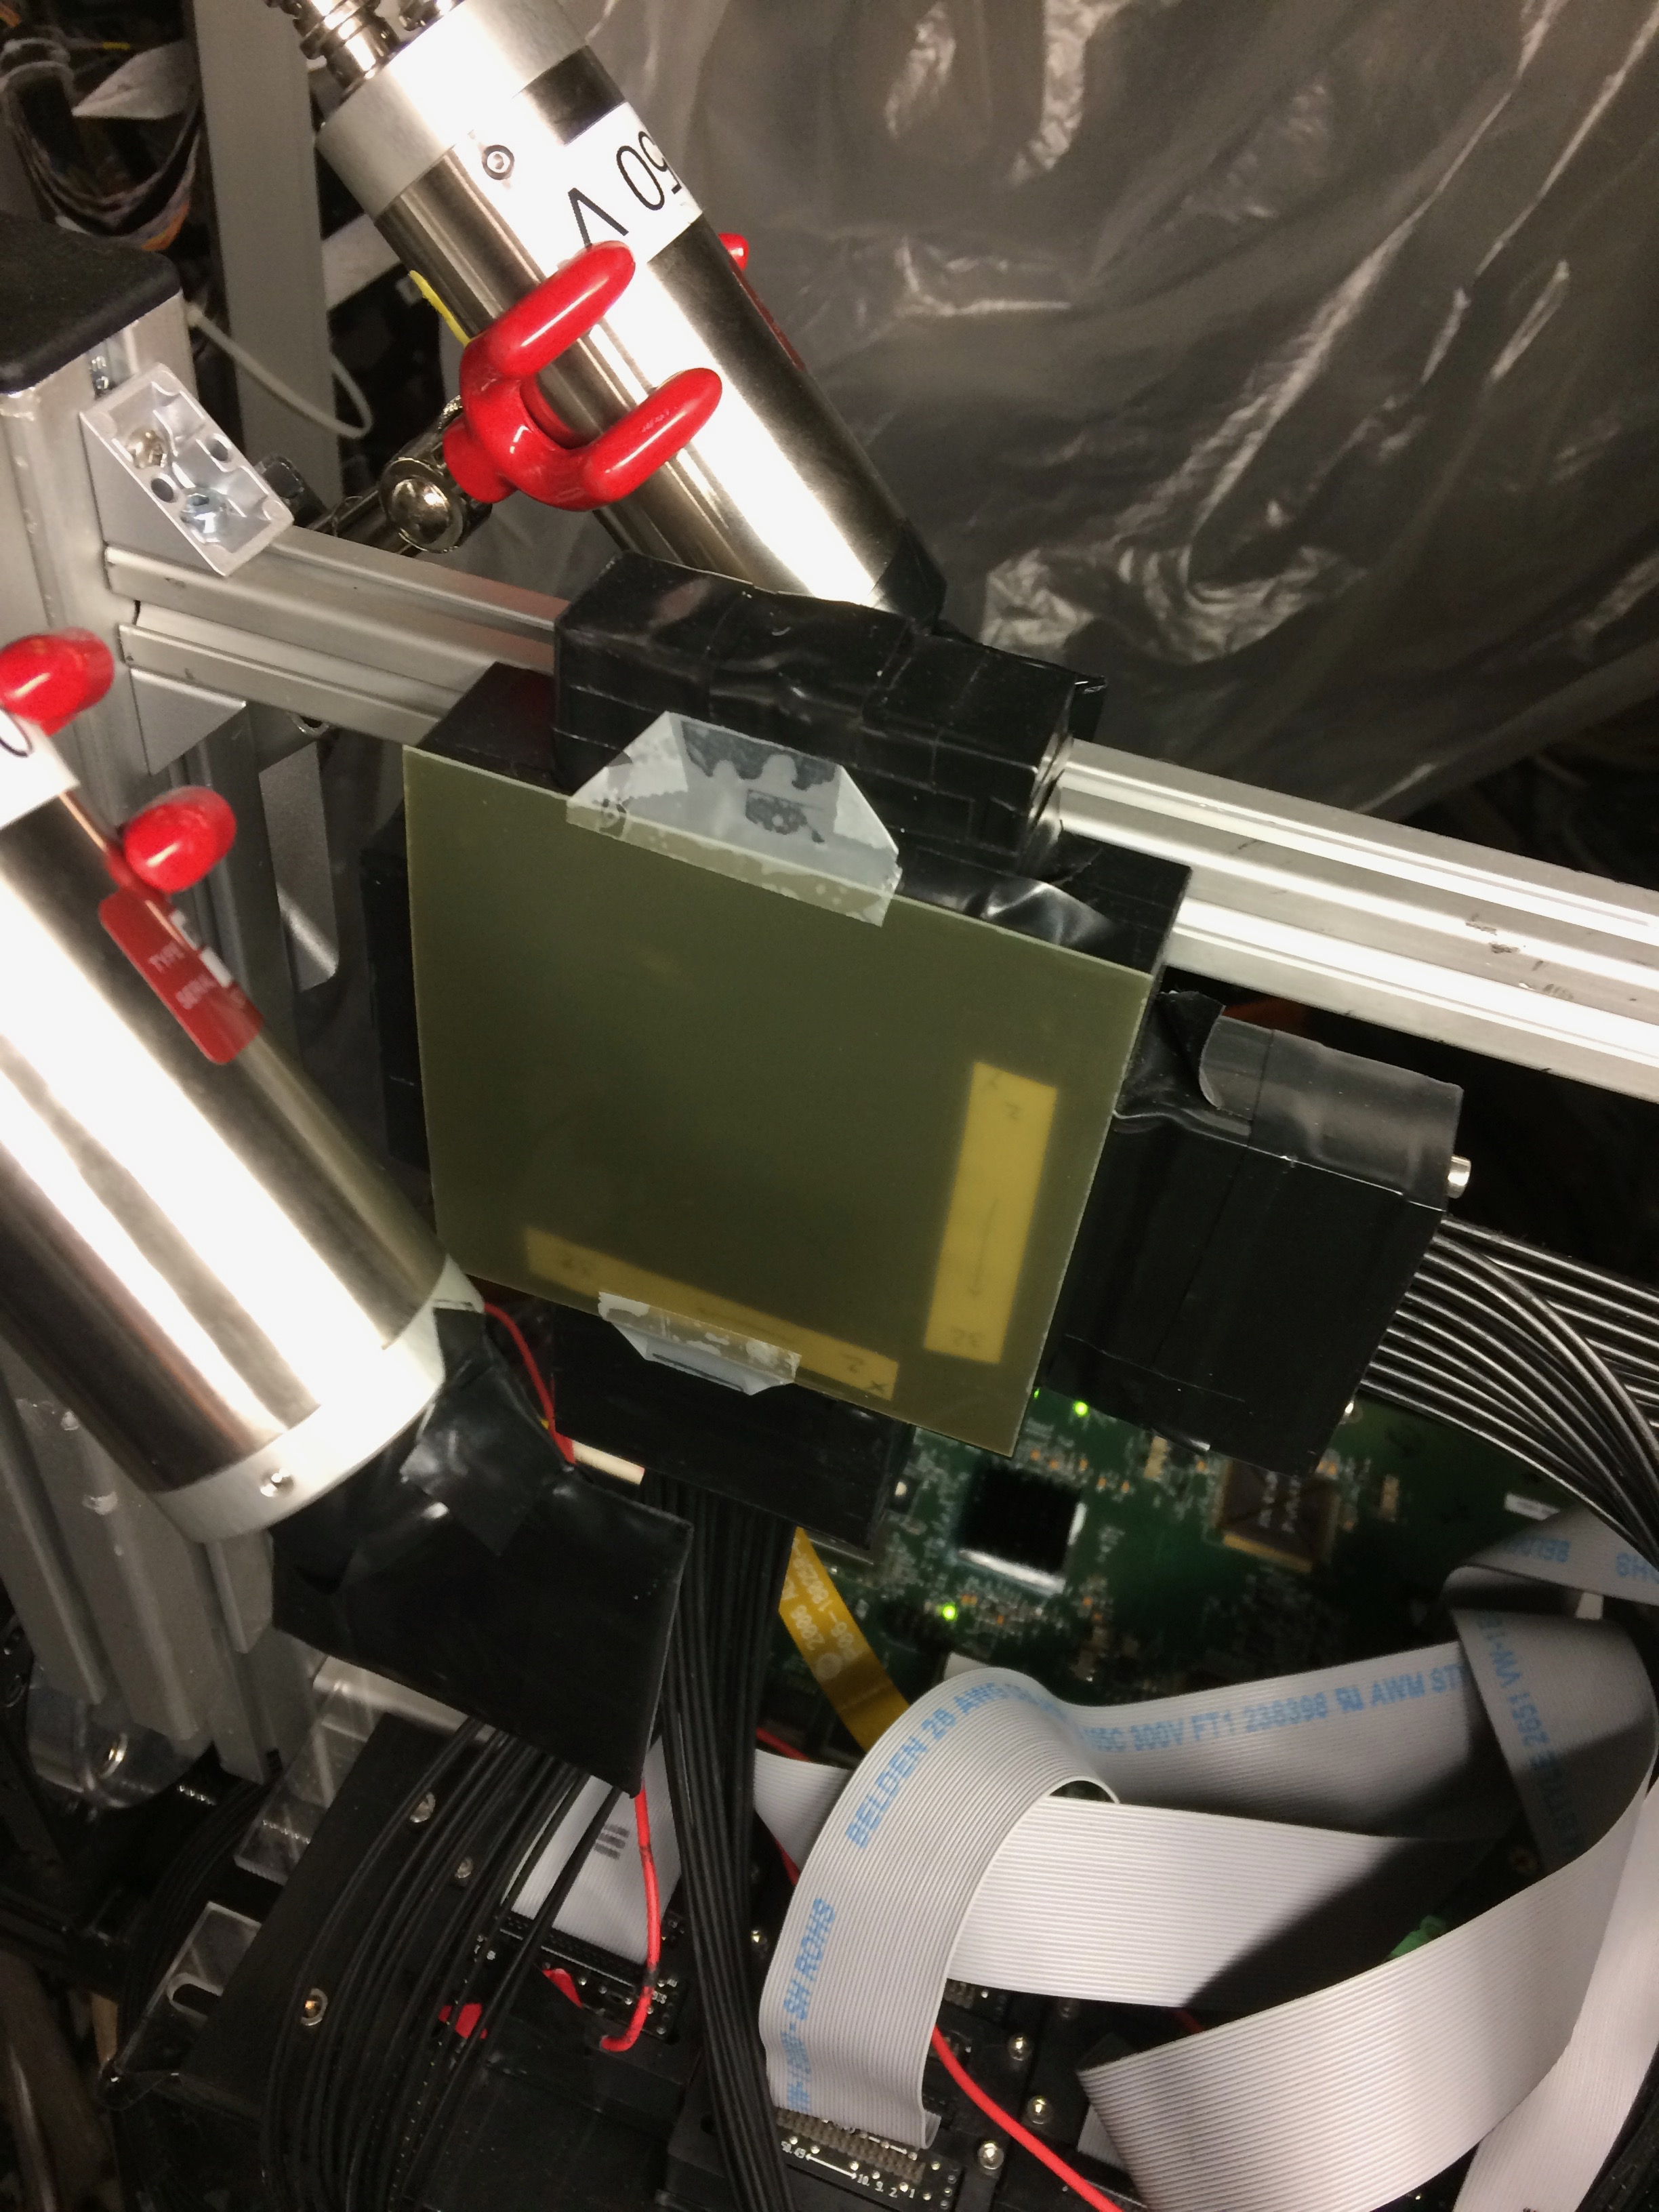
\includegraphics[width=0.9\textwidth]{03_GraphicFiles/chapter6_BeamTests/Nice_May2018/IMG_5170.jpg}
\caption{GAFchromic film fixed on the entrance surface hodoscope to record the beam shape at the hodoscope position.}
\label{chap6::fig::May_HodoFilm}
\end{subfigure}
\begin{subfigure}[t]{.5\textwidth}
\centering
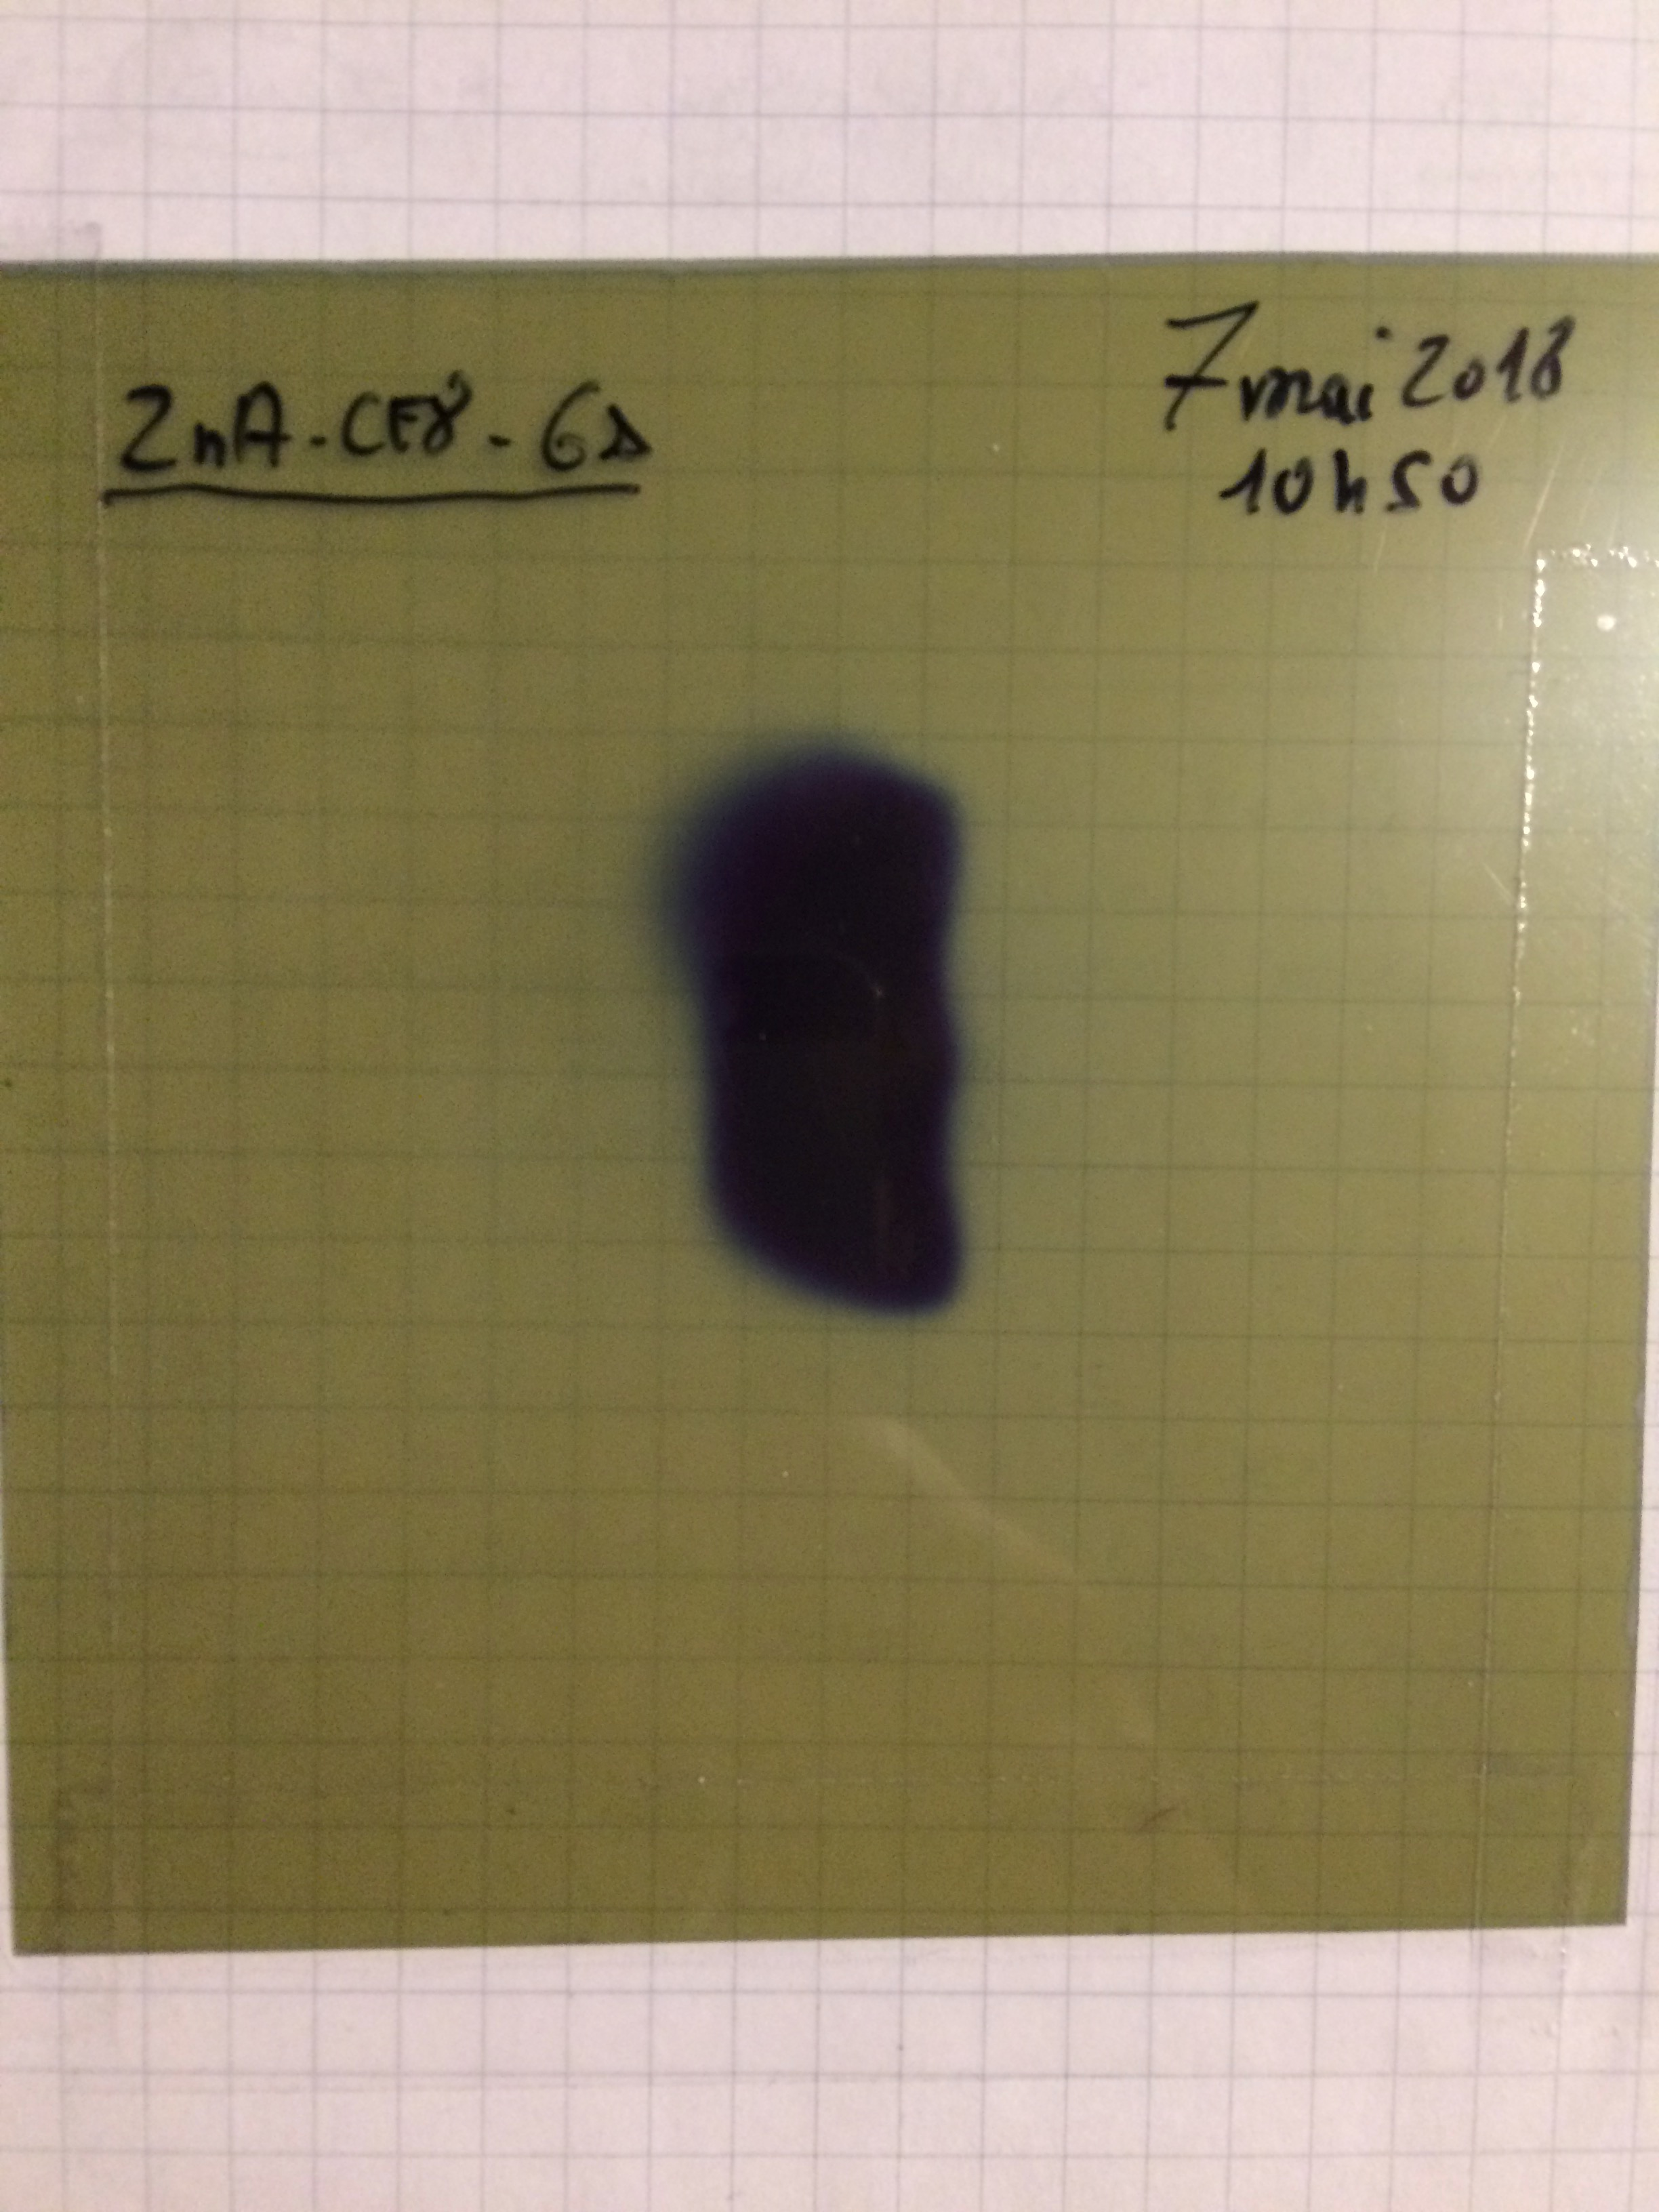
\includegraphics[width=0.9\textwidth]{03_GraphicFiles/chapter6_BeamTests/Nice_May2018/IMG_5849.JPG}	
\caption{Beam shape recorded with a 6~s irradiation at 2~nA beam intensity by a GAFchromic film fixed on the entrance surface of the hodoscope.}
\label{chap6::fig::May_HodoFilmBeam}
\end{subfigure}
\caption{Setup and result of a preliminary irradiation performed to estimate the beam shape at the hodoscope position.}
\label{chap6::fig::May_HodoGAFChrom}
\end{figure}

\subsection{Experimental results}\label{chap6::subsec::mayResults} 
After the tuning of the working parameters (plastic scintillators power supply and threshold, hodoscope \glspl{pm} power supply, \gls{fe} board threshold and gain of the two \glspl{asic}), our intensity monitoring system has been calibrated with the Faraday cage from very low intensities up to clinical intensities. In the following, we will refer to the intensity as a detection rate, measured by the hodoscope monitoring system based on the \gls{fe} board read out, which has been verified to be consistent with such a calibration.
Several test runs have been performed to verify all the acquisition and monitoring features, and to tune the beam intensity, which has been fixed to obtain an initial rate of detected external trigger signals (given by the coincidence of the two plastic scintillators on beam) of about 23~kHz and a corresponding detection rate on the hodoscope of 17~kHz in AND configuration.
As mentioned, the hodoscope detection efficiency has been tested at increasing beam intensity in the range 23-280~kHz of external trigger rate. The efficiency, expressed as percentage rate of recorded events with respect to the trigger counts, is reported as a function of the beam intensity in \figurename~\ref{chap6::fig::May_HodoEffInt}. The efficiency has been evaluated for the two hodoscope working modes (AND and OR). Even if in AND configuration the hodoscope is supposed to record only events with a coincidence between horizontal (x) and vertical (y) fiber planes, single plane events are also recorded; this issue is discussed in section~\ref{chap6::subsec::mayDiscussion}. For this reason, both the single plane and coincidence event detection efficiency are reported in \figurename~\ref{chap6::fig::May_HodoEffInt} for the two working modes of the hodoscope triggered by the external scintillator coincidence signal. In OR configuration, the horizontal-vertical plane coincidences are reconstructed at the analysis stage. Acquisition problems occurred at high trigger rate in hodoscope OR configuration, so that the data point at 280~kHz is missing for the OR configuration curves. 

\begin{figure}[!htbp]
\centering
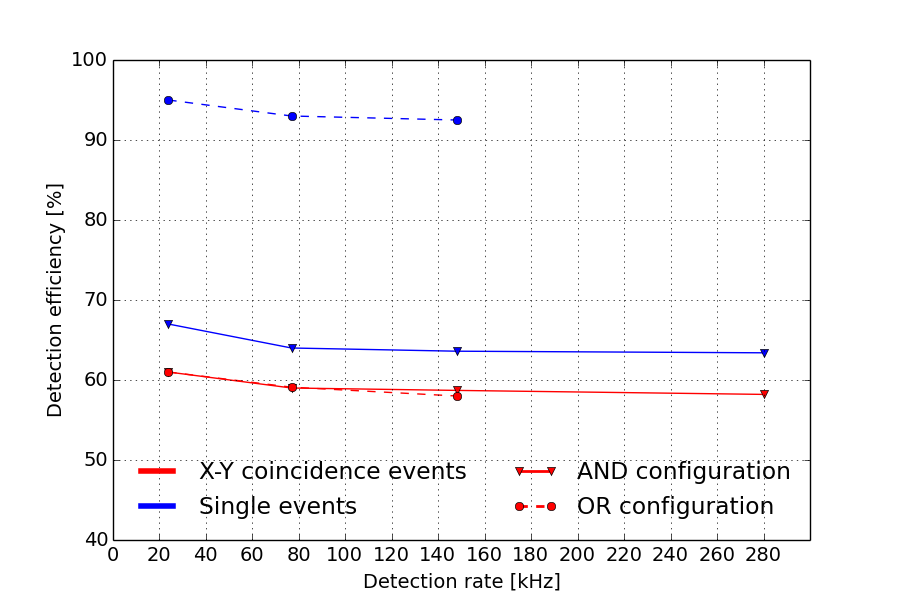
\includegraphics[width=0.7\textwidth]{03_GraphicFiles/chapter6_BeamTests/Nice_May2018/MAY_Eff_intensity.png}
\caption{Hodoscope detection efficiency as a function of the trigger detected rate for the different acquisition modes. The solid lines corresponds to acquisitions with the hodoscope in AND configuration, the dashed lines to the OR configuration. Red curves represent events with coincidence of horizontal (X) and vertical (Y) fiber planes, while blue curves include single plane and coincidence events.}
\label{chap6::fig::May_HodoEffInt}
\end{figure}

As expected, the detector efficiency slightly decreases for increasing beam intensity. The efficiency for events with coincidence of horizontal and vertical fiber planes ranges between 62 and 58\% and is compatible in AND and OR hodoscope working mode. An efficiency beyond 90\% over the whole beam intensity range has been obtained in OR configuration including both single plane and coincidence events. As mentioned, also in AND configuration single events are recorded and the efficiency for the detection of this kind of events is in the range 67-64\%. 

The hodoscope spatial and time performance have been studied with acquisitions with external trigger and AND of horizontal and vertical fibers configuration, at the lowest beam intensity provided during the test, corresponding to 23~kHz of trigger detection rate. 
In \figurename~\ref{chap6::fig::May_HodoMap2D} the two-dimensional beam profile collected by the hodoscope is shown. To be noticed that each plot bin corresponds to a single 1~mm fiber in the two spatial directions. The collected beam profile perfectly fits with the expectation, with a vertical extension of 30 fibers (30~mm), by considering twice the distance between the profile maximum and the top irradiated bin, and a horizontal extension of about 20 fibers (20~mm). The mono-dimensional profiles shown in \figurename~\ref{chap6::fig::May_Hodoprof1D} for the horizontal (left) and vertical (right) direction confirm the good spatial detection of the beam profile.     

\begin{figure}[!htbp]
\centering
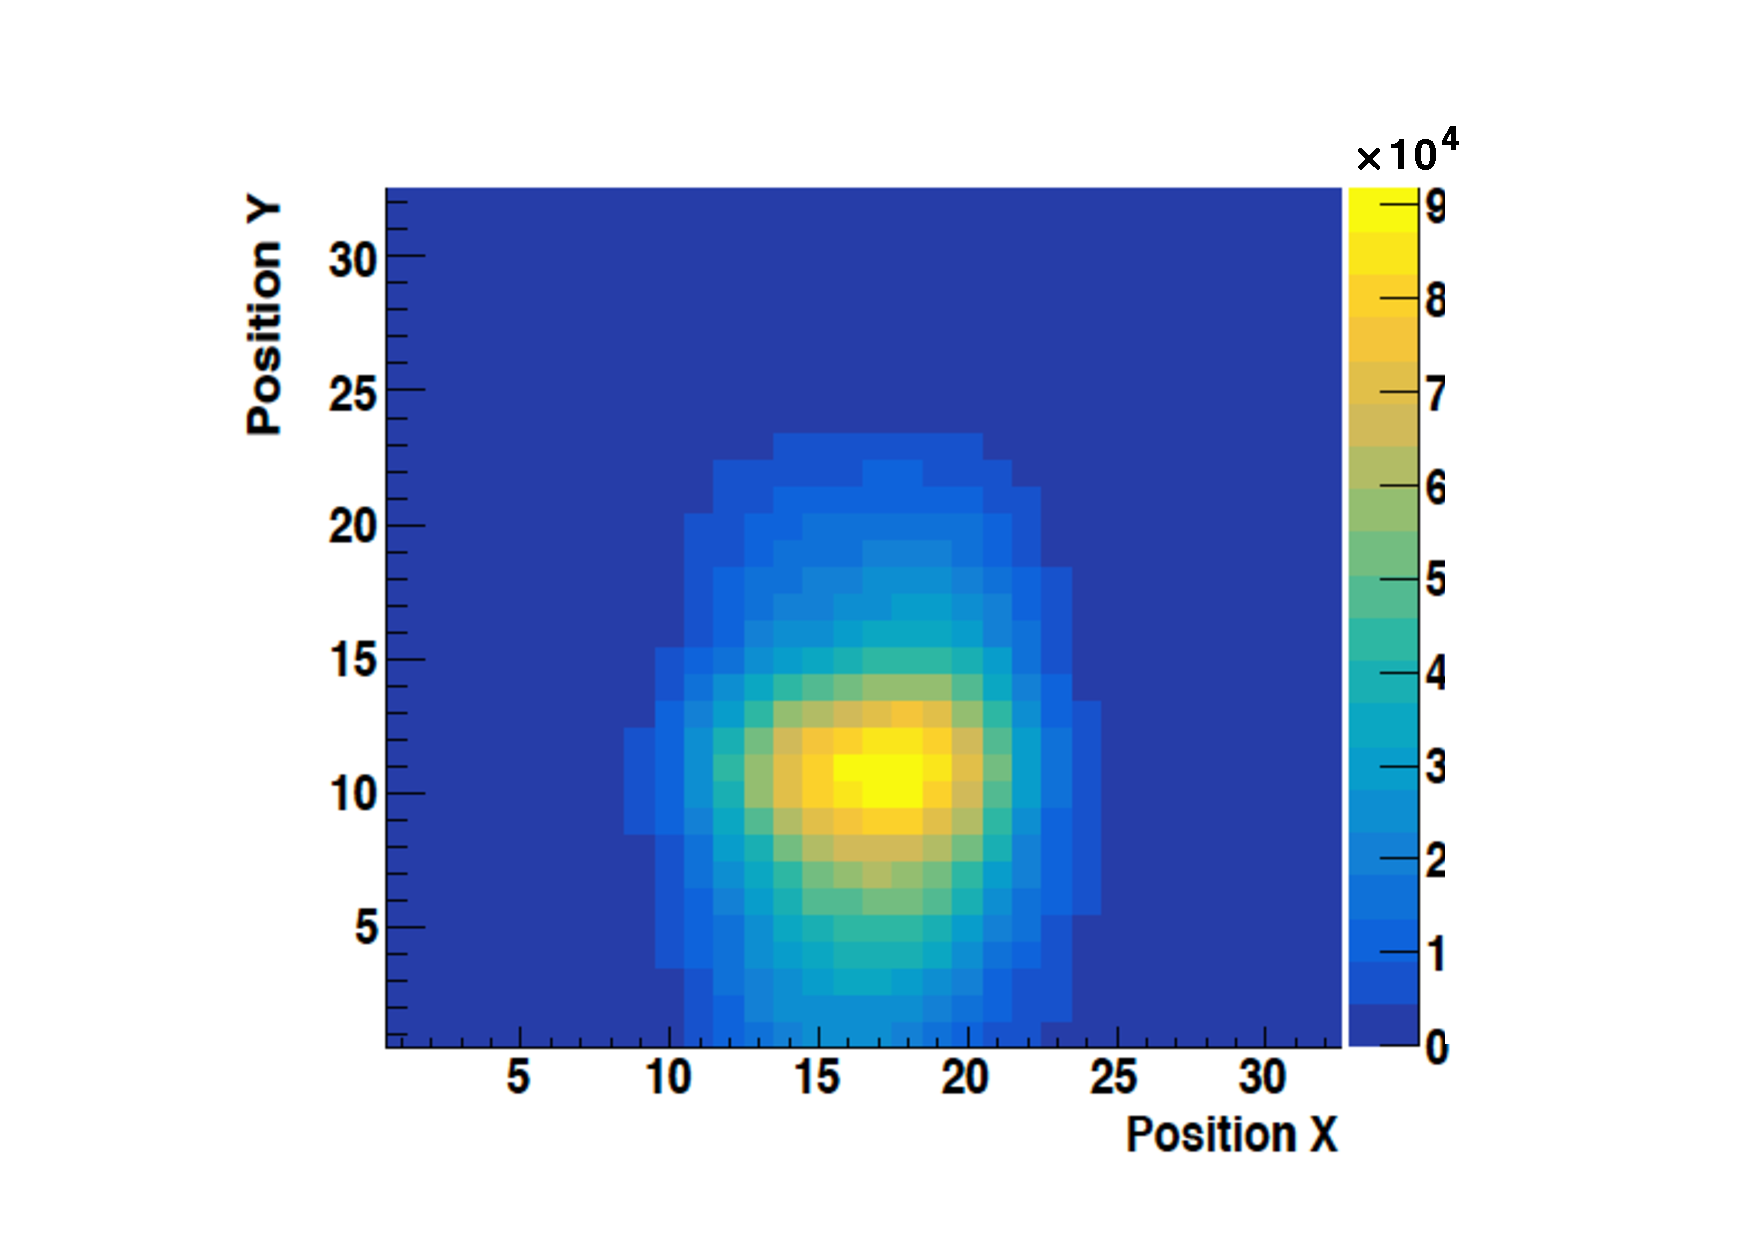
\includegraphics[width=0.8\textwidth]{03_GraphicFiles/chapter6_BeamTests/Nice_May2018/map2D.pdf}
\caption{Two dimensional beam profile recorded by the hodoscope. The bin size corresponds to the hodoscope scintillating fiber size (1~mm).}
\label{chap6::fig::May_HodoMap2D}
\end{figure}

\begin{figure}
\begin{subfigure}[t]{.5\textwidth}
\centering
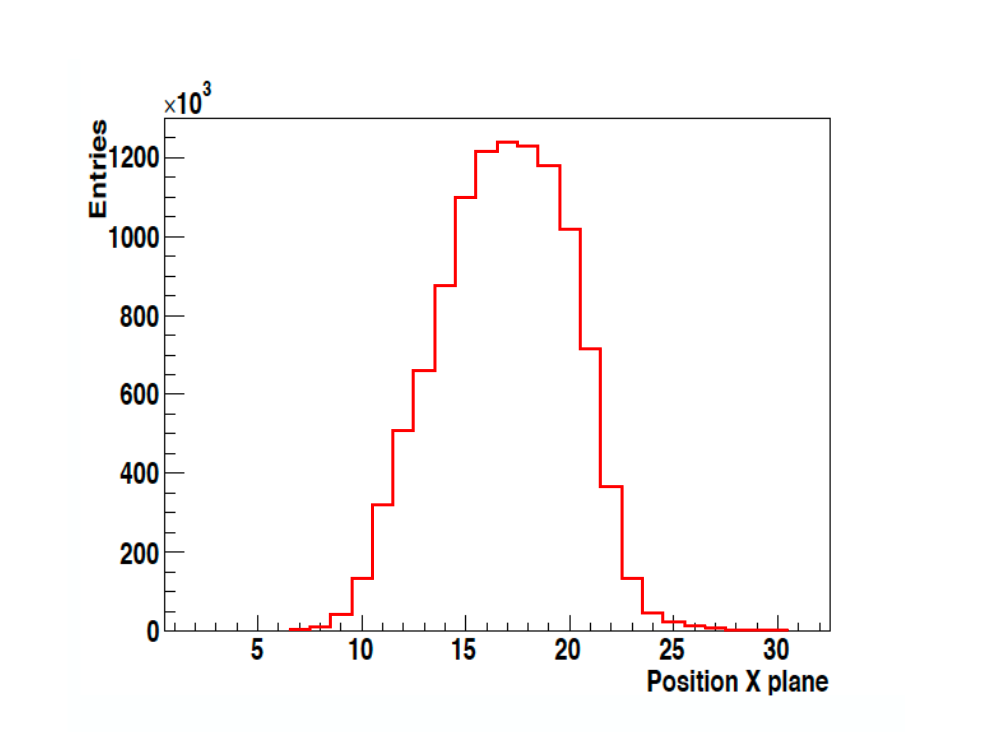
\includegraphics[width=1.1\textwidth]{03_GraphicFiles/chapter6_BeamTests/Nice_May2018/profileX.png}
\caption{Horizontal plane.}
\label{chap6::fig::May_HodoprofX}
\end{subfigure}
\begin{subfigure}[t]{.5\textwidth}
\centering
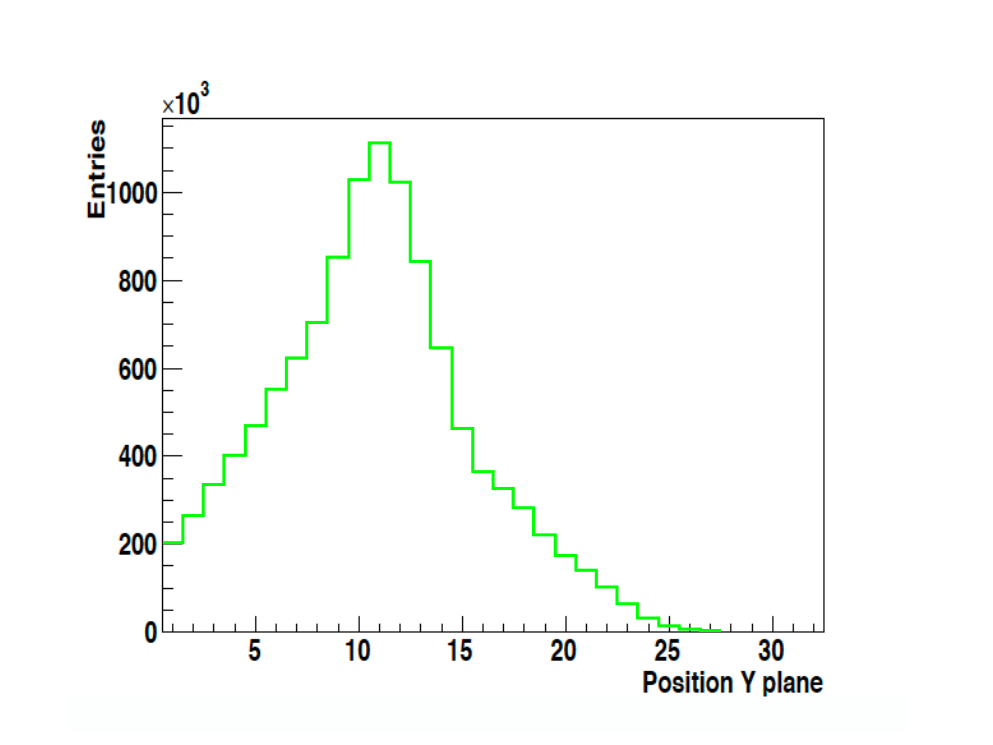
\includegraphics[width=1.1\textwidth]{03_GraphicFiles/chapter6_BeamTests/Nice_May2018/profileY.png}	
\caption{Vertical plane.}
\label{chap6::fig::May_HodoprofY}
\end{subfigure}
\caption{Mono-dimensional spatial profiles of the beam recorded by the hodoscope.}
\label{chap6::fig::May_Hodoprof1D}
\end{figure}

The spatial performance of the hodoscope are also determined by the number of fibers involved in each interaction. This parameter has been studied and the results are shown in \figurename~\ref{chap6::fig::May_HodoClusters} for the two axes. As expected, in most of the interactions one single fiber per axis is involved. However, a significant amount of events shows two or more fibers involved in at least one of the two axes. Moreover, since the acquisition was performed in hodoscope AND mode, at least one fiber per axis should be mandatory to validate the event and send it to the \gls{utca} for the acquisition. The presence of events with no fibers hit in one of the two planes confirms the aforementioned problem, discussed in section~\ref{chap6::subsec::mayDiscussion}. 
 
\begin{figure}
\begin{subfigure}[t]{.5\textwidth}
\centering
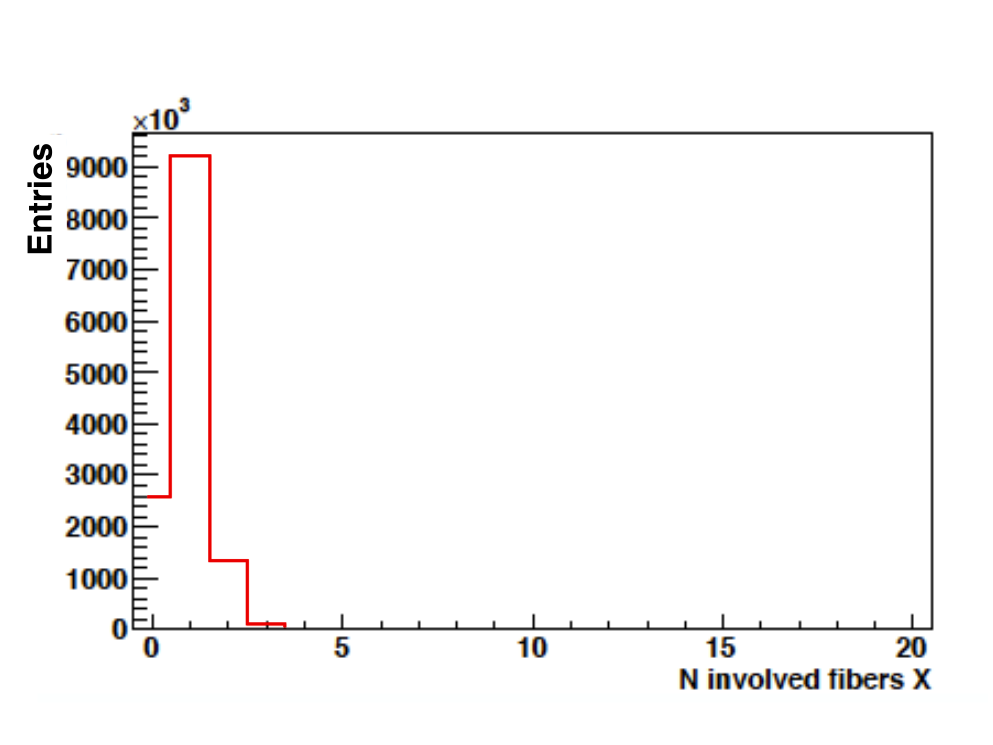
\includegraphics[width=1.\textwidth]{03_GraphicFiles/chapter6_BeamTests/Nice_May2018/clusterX.png}
\caption{Horizontal plane.}
\label{chap6::fig::May_HodoClusX}
\end{subfigure}
\begin{subfigure}[t]{.5\textwidth}
\centering
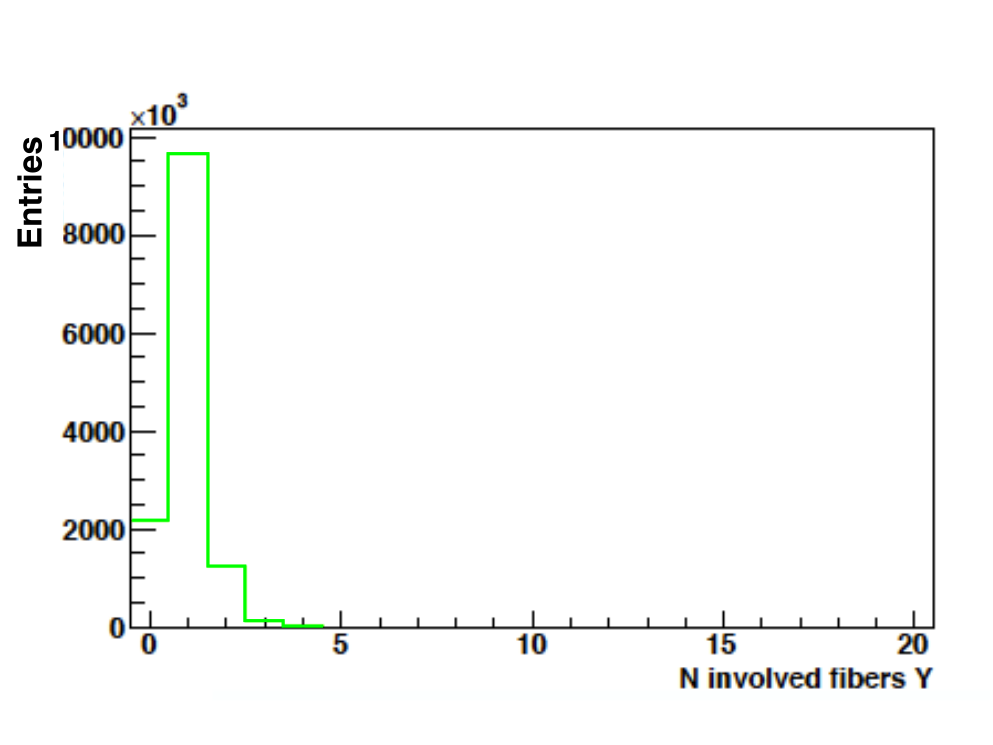
\includegraphics[width=1.\textwidth]{03_GraphicFiles/chapter6_BeamTests/Nice_May2018/clusterY.png}	
\caption{Vertical plane.}
\label{chap6::fig::May_HodoClusY}
\end{subfigure}
\caption{Number of involved fibers per event recorded by the hodoscope for the two planes.}
\label{chap6::fig::May_HodoClusters}
\end{figure}

The hodoscope timing performance has been also analyzed with this low beam intensity run. The absolute time (with respect to the board internal clock), is measured separately for the two fiber planes and for the trigger signal. Concerning the fiber plane time, it corresponds to the arrival time of the first event detected in the defined time coincidence window. The coincidence window was fixed, for this test, to 3 board internal clock counts, corresponding to 24~ns. Given the problem detected in the previous analysis, the timing performance analysis is limited to coincidence events selected at the data processing stage.
\figurename~\ref{chap6::fig::May_HodoDeltaT} shows the distributions of the measured time for the two fiber planes (horizontal - left - and vertical - right). The distribution \gls{fwhm} widths are 6.8~ns and 5.3~ns for the x and y plane, respectively. 

\begin{figure}
\begin{subfigure}[t]{.5\textwidth}
\centering
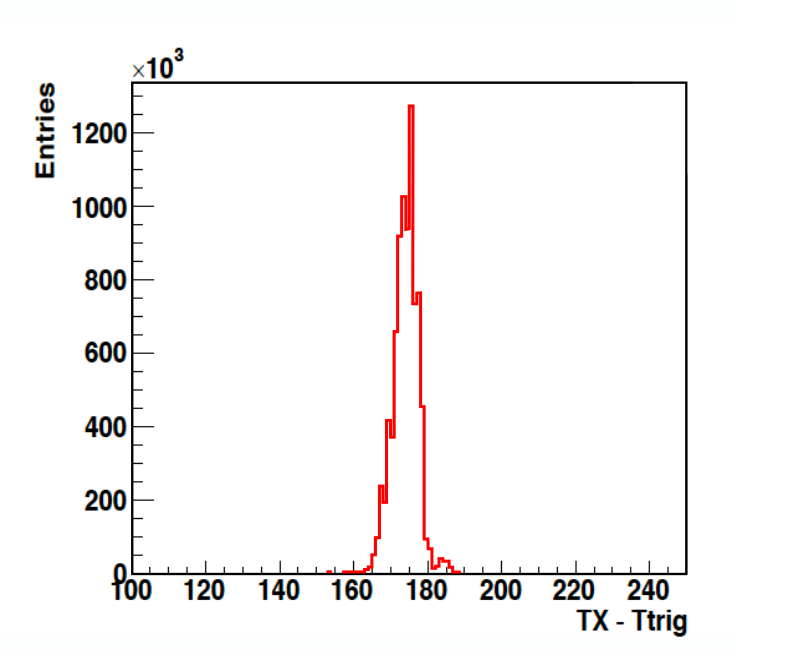
\includegraphics[width=1.1\textwidth, trim={0 0.6cm 0 0} , clip=true]{03_GraphicFiles/chapter6_BeamTests/Nice_May2018/TX-Ttrig.png}
\caption{Horizontal plane.}
\label{chap6::fig::May_HododTx}
\end{subfigure}
\begin{subfigure}[t]{.5\textwidth}
\centering
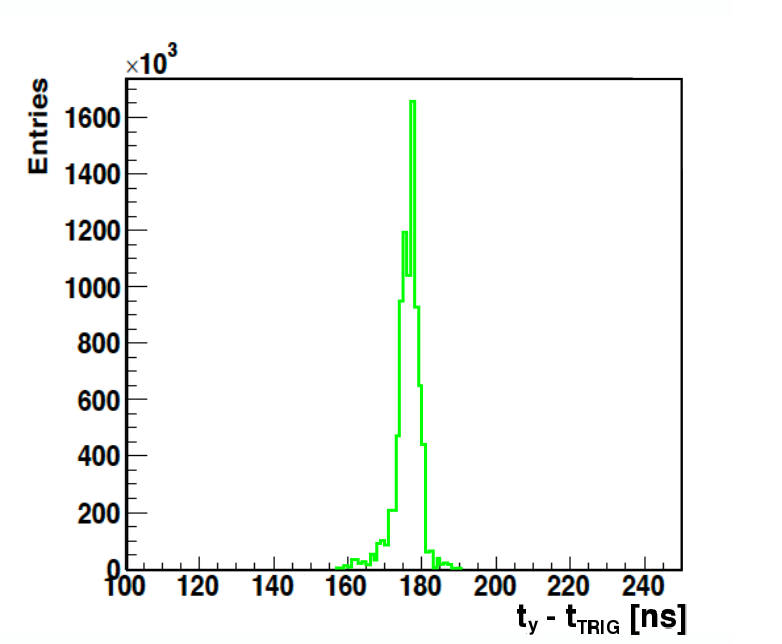
\includegraphics[width=1.1\textwidth]{03_GraphicFiles/chapter6_BeamTests/Nice_May2018/TY-Ttrig.png}	
\caption{Vertical plane.}
\label{chap6::fig::May_HododTy}
\end{subfigure}
\caption{Distribution of the time difference between the trigger arrival time and the time measured by the two hodoscope fiber planes.}
\label{chap6::fig::May_HodoDeltaT}
\end{figure}

The distribution of the measured absolute time difference between the two fiber planes has also been studied and is reported in \figurename~\ref{chap6::fig::May_HodoDeltaTFibers}. The experimental distribution has a mean value of 2.4~ns and a width \gls{fwhm} of 3.5~ns.

\begin{figure}[!htbp]
\centering
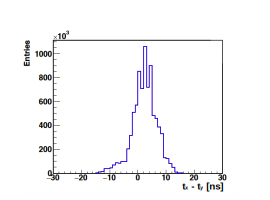
\includegraphics[width=0.75\textwidth]{03_GraphicFiles/chapter6_BeamTests/Nice_May2018/TX-TY.png}
\caption{Distribution of the time difference between the two hodoscope fiber planes for horizontal-vertical plane coincidence events.}
\label{chap6::fig::May_HodoDeltaTFibers}
\end{figure}

\subsection{Discussion}\label{chap6::subsec::mayDiscussion} 

After a preliminary test performed in December 2017, in May 2018 the 32$\times$32 scintillating fiber hodoscope has been tested on beam for the first time with the final \gls{utca}-based acquisition system. The promising results presented in the previous section allowed to estimate the hodoscope performance, highlight the main issues for what concerns the detector, the electronics boards and the acquisition system, and plan the development advancements.
In particular, it has been shown that:
\begin{itemize}
\item a detection efficiency beyond 90\% can be achieved at the explored beam intensity;
\item the hodoscope spatial response it satisfactory and the beam profile has been correctly recorded;
\item in most of the events, 1 or 2 fibers per detection plane are involved;
\item the time response is limited to a 6-7~ns time window.
\end{itemize}

Notwithstanding the encouraging results, the \gls{fe} board and acquisition firmware and software showed some issues during this first test. In particular, the AND configuration showed an unexpected behavior. As mentioned, with this working mode, only events with time coincidence between the horizontal and the vertical fiber planes should be recorded, but also non-coincidence events have been collected. 
Some laboratory tests have been performed after the end of the beam test campaign, and a possible explanation has been found in the data processing at the hodoscope \gls{fe} board level. The analog signals emerging from the hodoscope read-out \glspl{pm} are collected on the board and converted to logic with the application of a fixed threshold. The logic signal time width depends on the time-over-threshold of the analog signal, so that low amplitude analog signals can trigger the acquisition but result in very short logic output. If the AND function implemented on the board to verify the coincidence takes more time than the logic signal width, the coincidence can be triggered but the logic signal related to the hit fiber can be lost. 
This effect could explain the presence of single plane interaction also in AND working mode. In addition, this effect could also be the cause of the low efficiency in AND configuration (below 60\%), and, in general, for the detection of coincidences between the two fiber perpendicular planes, shown in figure~\ref{chap6::fig::May_HodoEffInt}. 
The presented timing performance have been obtained with a preliminary time calculation method. the time measurement features implemented on the \gls{fe} board was still under development at the moment of testing, and the trigger arrival time was measured according to the internal board clock. A dedicated clock with 250~ps resolution was already implemented on the \gls{fe} board for the hodoscope fiber time measurement. The installation of a dedicated \gls{tdc} on the card for the trigger channel is foreseen for the final configuration, for which the \gls{tof} between the absorber and the hodoscope interactions will be measured. The trigger time measurement method affected the time resolution which is below the expectations. The distribution of the time difference between the fibers in the two detection planes was expected to be centered in $t_{x}-t_{y} = 0$, and its width was expected to reflect the hodoscope time resolution, given the superior resolution of the reference clock (250~ps). The obtained results (3.5~ns \gls{fwhm} width, mean value of 2.4~ns) are not satisfactory. This degraded performance is probably due to the time measurement method, which selects the first event in the time coincidence window as time reference. In case of background contamination, un-correlated background events collected in the coincidence window degrades the time resolution. Background events are also the identified cause of events with more than one fiber hit per plane. The data analysis revealed a large amount of events with un-correlated fibers hit in coincidence (spatially separated by more than 2~mm), clear evidence of background contamination.
The planned improvements to the firmware of the hodoscope \gls{fe} boards and a fine tuning of the board working parameters are expected to solve the highlighted issues. In particular, a gain and a threshold are fixed on the hodoscope board \gls{asic} for each read-out channel (each fiber), and an appropriate calibration of their values will probably allow to obtain analog signals with sufficient amplitude to result in larger logic signal, able to trigger the coincidence read-out and be transferred to the data acquisition with non-zero values. This should improve the overall efficiency of the system and guarantee the correct functionality of the AND acquisition setting. Moreover, the proper threshold should reduce the background contamination, thus improving the timing and spatial performance.  
An automatic calibration method has been developed in the summer 2018 in collaboration with an internship student, and applied to characterize the hodoscope board \gls{asic} behavior for background measurements. The same strategy will be applied during a dedicated beam test before the end of 2018 to define the hodoscope optimal working parameters for the monitoring of proton beams. A second dedicated test will be then necessary for the characterization of the hodoscope with carbon ions, which are expected to induce different response due to an increased energy deposit in the scintillating fibers.   
Finally, before the end of this first test, the \gls{utca} trigger capabilities have been tested with two hodoscope cards to mimic the coupling of two camera components. This first attempt allowed to create the bases for the firmware and electronics development of the following months, which aimed to prepare the system for the test of a multi-collimated camera configuration, i.e. the coupling of hodoscope and absorber, performed in September 2018 and described in section~\ref{chap6::sec::september2018}. 


\section{Collimated camera: September 2018}\label{chap6::sec::september2018}

Following the hodoscope test performed in May 2018, the \gls{ipnl} electronics group focused on the integration of the absorber block read-out in the \gls{utca} acquisition system and on the validation of the trigger \gls{utca} handling. The generation of trigger signals by the \gls{bgo} blocks has been tested at the \gls{ipnl} with gamma sources, and the final integration of hodoscope and absorber has been tested on beam in September 2018. 
6 \gls{bgo} blocks composed the minimal multi-collimated camera absorber, read-out by a single \gls{asm} board. As described in chapter~\ref{chap::3}, a \gls{fe} card is connected to each block: it is in charge of splitting the power supply to the four \glspl{pm} and sending the collected signals to the read-out \gls{asm} board. Each \gls{asm} board has 24 channels, so that it is designed for the read-out of a maximum of 6 blocks. The data are sampled at the selected frequency (up to 5 \gls{gsps} for 1024 samples). The integral of each signal (total collected charge) will be calculated on the card and directly sent to the acquisition system in the final camera acquisition configuration, while a test operating mode has been used for this preliminary beam measurements, with all the samples of each signal sent to the acquisition and stored (see section~\ref{chapappA::subsec::absDataFormat}). The selected sampling frequency has been 1 \gls{gsps}, with 1~\charmus signal width digitized. 
One of the two identical tungsten collimators described in chapter~\ref{chap::3} has been placed in front of the absorber blocks. The 32$\times$32 fiber hodoscope has been used for the trigger generation tests and the first \gls{tof} measurements.
A schematic view of the measurement setup is shown in \figurename~\ref{chap6::fig::September_DAQscheme} from top view. 

\begin{figure}[!htbp]
\centering
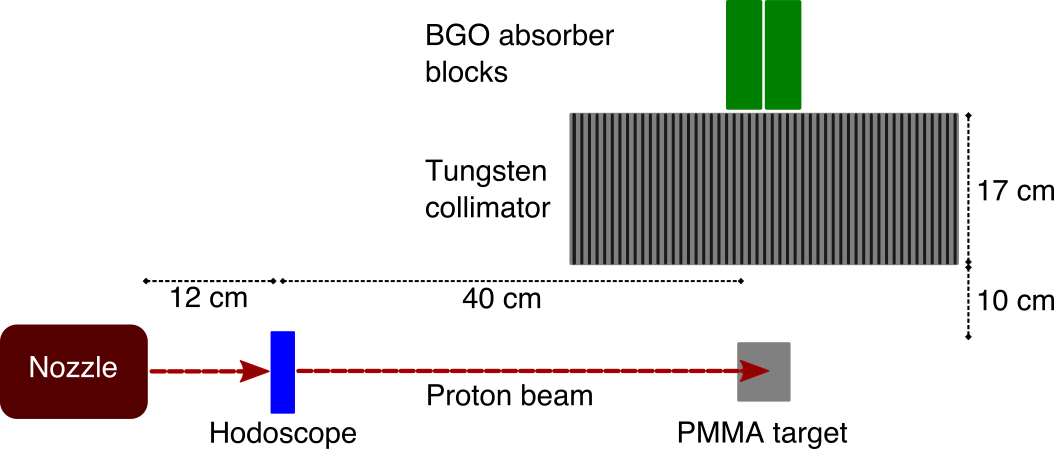
\includegraphics[width=0.9\textwidth]{03_GraphicFiles/chapter6_BeamTests/Nice_September2018/1Dscheme.png}
\caption{Schematic view of the hodoscope and the multi-collimated camera setup for the beam test at \gls{cal}.}
\label{chap6::fig::September_DAQscheme}
\end{figure}

The hodoscope, mounted on its remotely controlled support, has been set at a distance of 12~cm from the beam nozzle, and aligned to the beam exit. Two \gls{pmma} 5~cm side cubes have been used as target, aligned to the beam line and set 40~cm far from the hodoscope center. The two targets have been disposed one on top of the other to completely stop the beam, which has a spot size increasing with the distance from the nozzle. GAFchromic films have been fixed to the hodoscope entrance surface and to the top target cube, and a 10~s irradiation at approximately 1~nA of beam current allowed to record the beam spot size in the two positions. The results are shown in \figurename~\ref{chap6::fig::September_beamSize}. The beam size close to the nozzle (on the hodoscope surface) is approximately the same as in the previous test (see \figurename~\ref{chap6::fig::May_HodoFilmBeam}), with a 1.5$\times$3~cm$^2$ rectangular shape. The beam spread is evident at the target position, where the spot has ellipsoidal shape, with axes of approximately 5 and 4 cm. The multi-collimated camera was set at 90\textdegree ~with respect to the beam direction, with the collimator entrance surface at a distance of 10~cm from the target. The 6 absorber blocks are in contact to the collimator back face, and disposed in two columns of three blocks each within the custom mechanical support built at \gls{ipnl}, with the center of the column on the nozzle side aligned with the target entrance face. A picture of the complete setup is shown in \figurename~\ref{chap6::fig::September_SetupPicture}, while detailed side and front-views of the multi-collimated camera are given in \figurename~\ref{chap6::fig::September_SetupCameraDetails}.

\begin{figure}[!htbp]
\begin{subfigure}[t]{.5\textwidth}
\centering
\includegraphics[width=1.\textwidth]{03_GraphicFiles/chapter6_BeamTests/Nice_September2018/hodo_target_beam.png}
\caption{Beam size recorder with GAFchromic films on the hodoscope and \gls{pmma} target entrance surfaces.}
\label{chap6::fig::September_beamSize}
\end{subfigure}
\begin{subfigure}[t]{.5\textwidth}
\centering
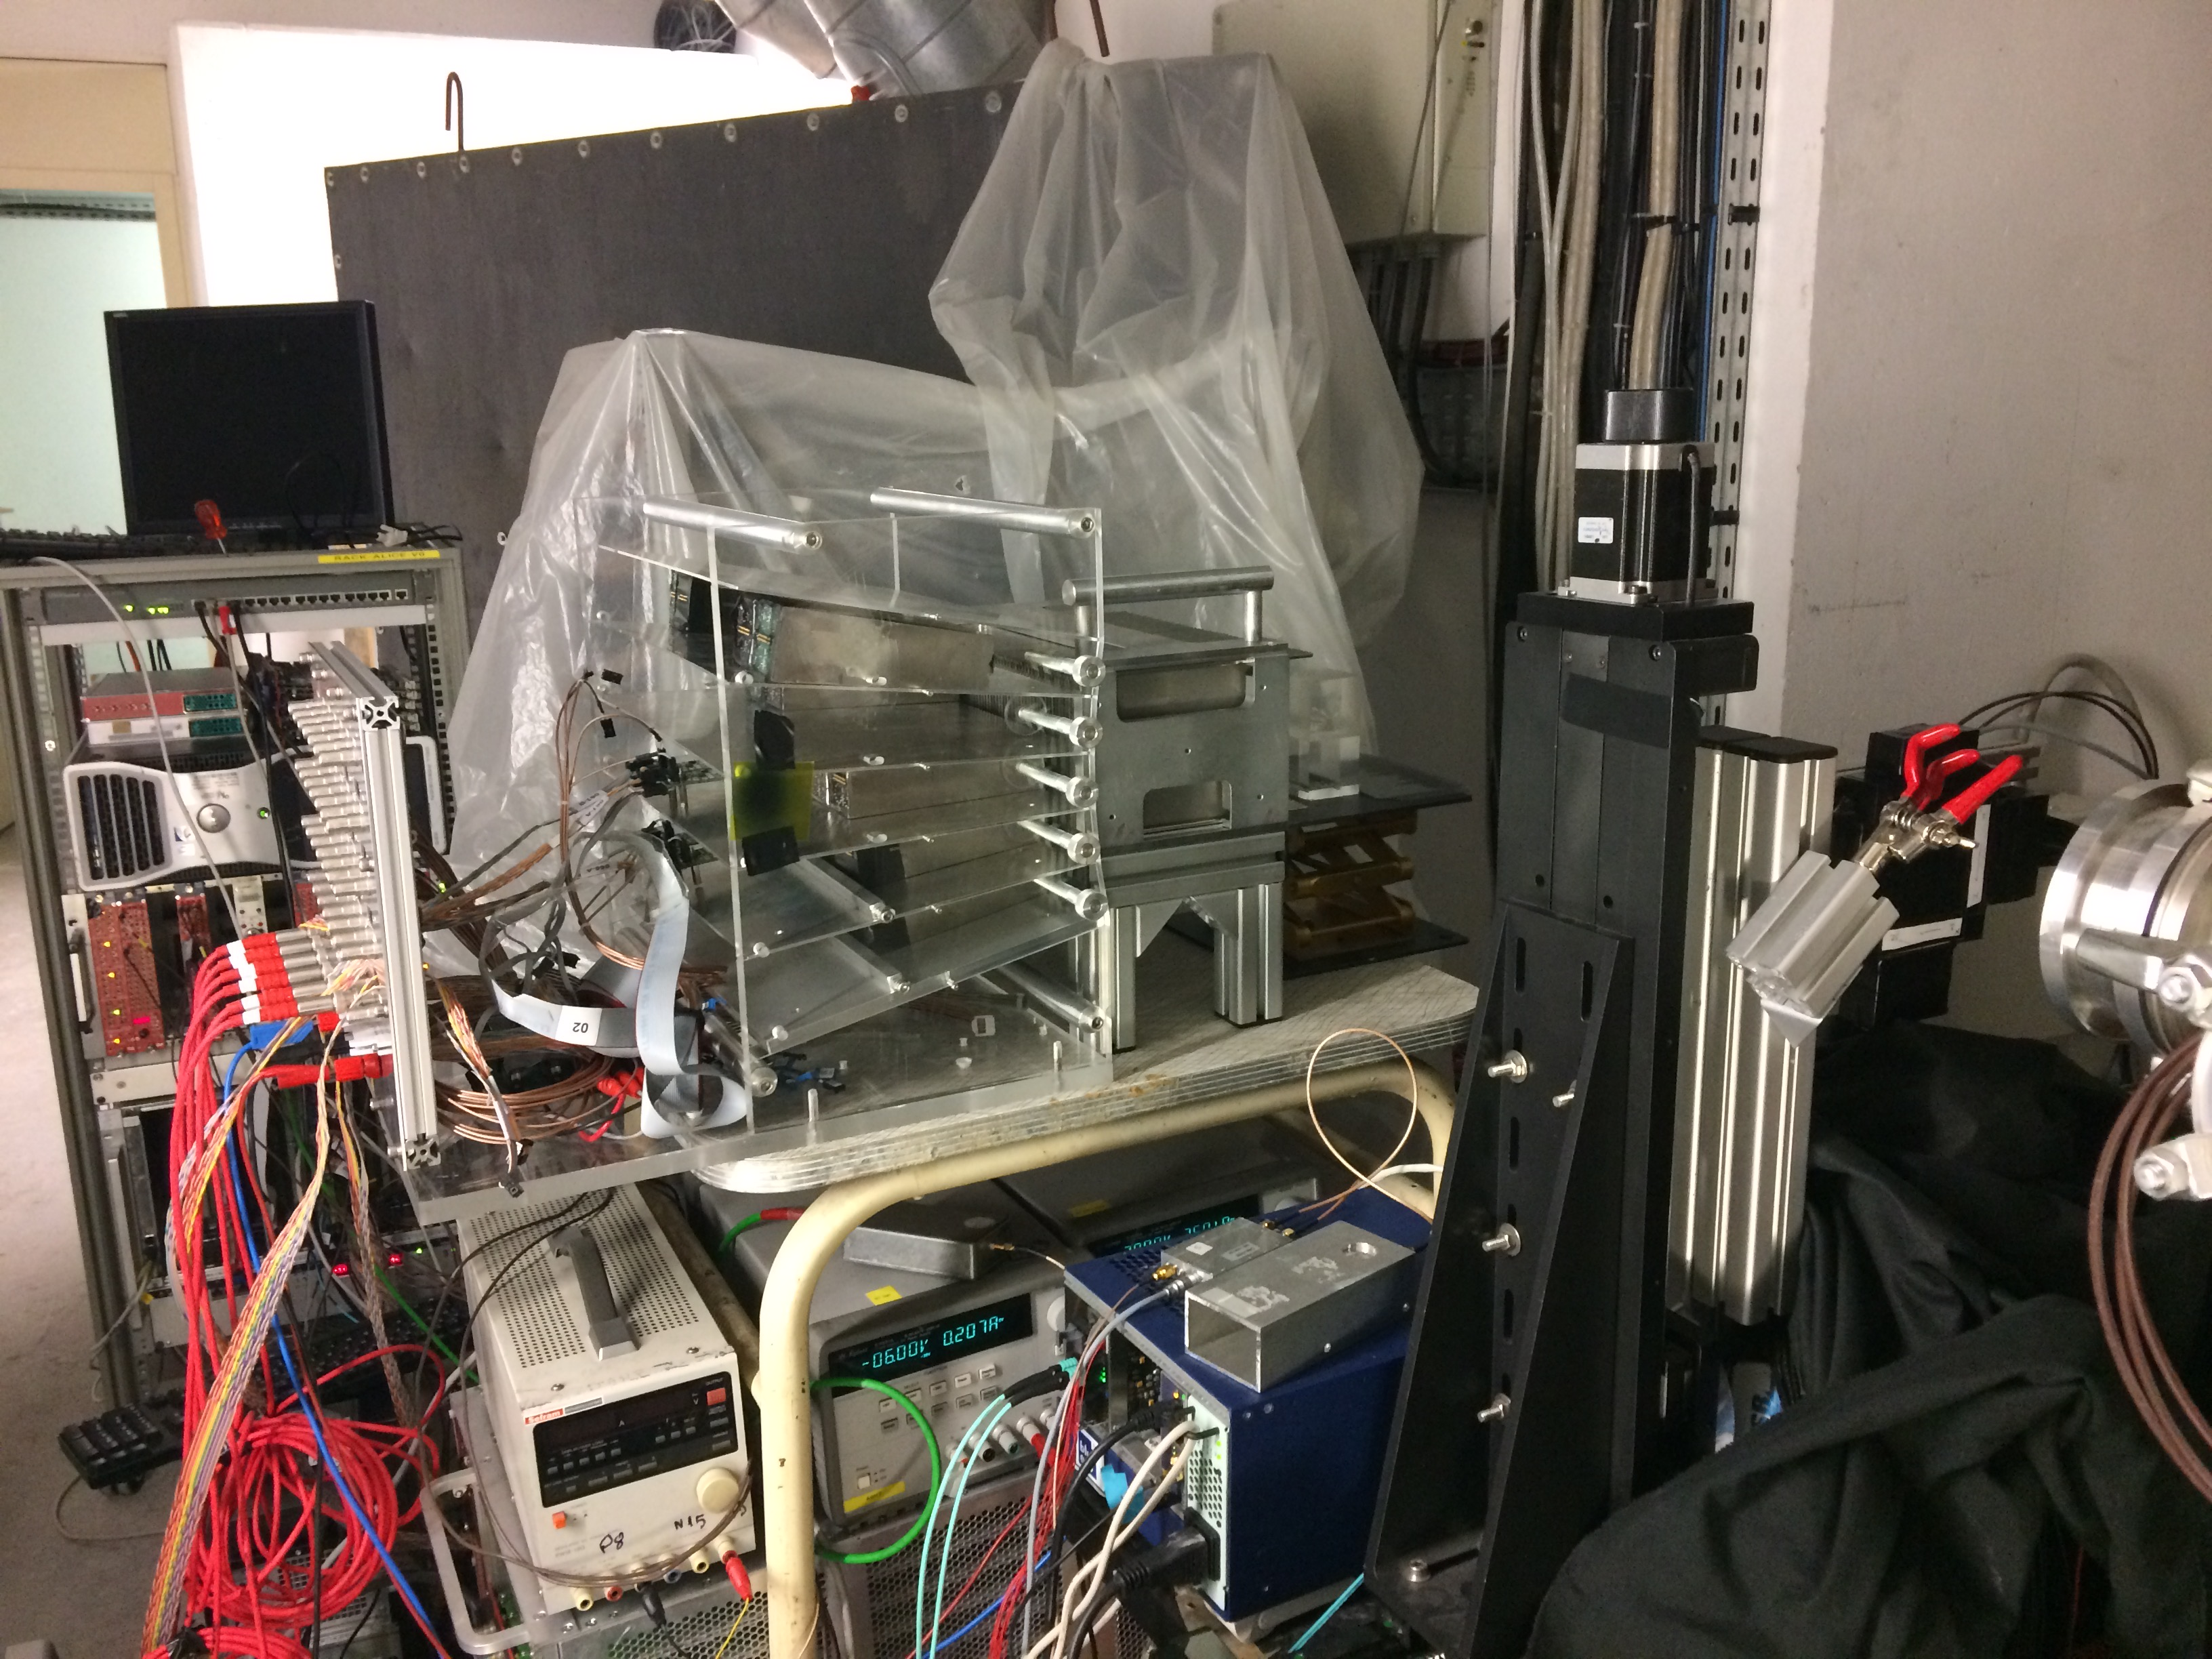
\includegraphics[width=1.\textwidth]{03_GraphicFiles/chapter6_BeamTests/Nice_September2018/Setup_withColl_withHodo.jpg}	
\caption{Beam test setup including the beam tagging hodoscope 12~cm far from the beam nozzle, the \gls{pmma} cubes (40~cm far from the hodoscope) used as target and set on a support with adjustable height, and multi-collimated camera at 90\textdegree ~with respect to the beam direction. The tungsten collimator entrance face is at 10~cm from the target, and the 6 absorber blocks are in contact with the collimator back face.}
\label{chap6::fig::September_SetupPicture}
\end{subfigure}
\caption{Beam size recorder with GAFchromic films (left) and complete setup of the hodoscope and multi-collimated camera test (right).}
\label{chap6::fig::September_SetupCamera}
\end{figure}

\begin{figure}[!htbp]
\begin{subfigure}[t]{.5\textwidth}
\centering
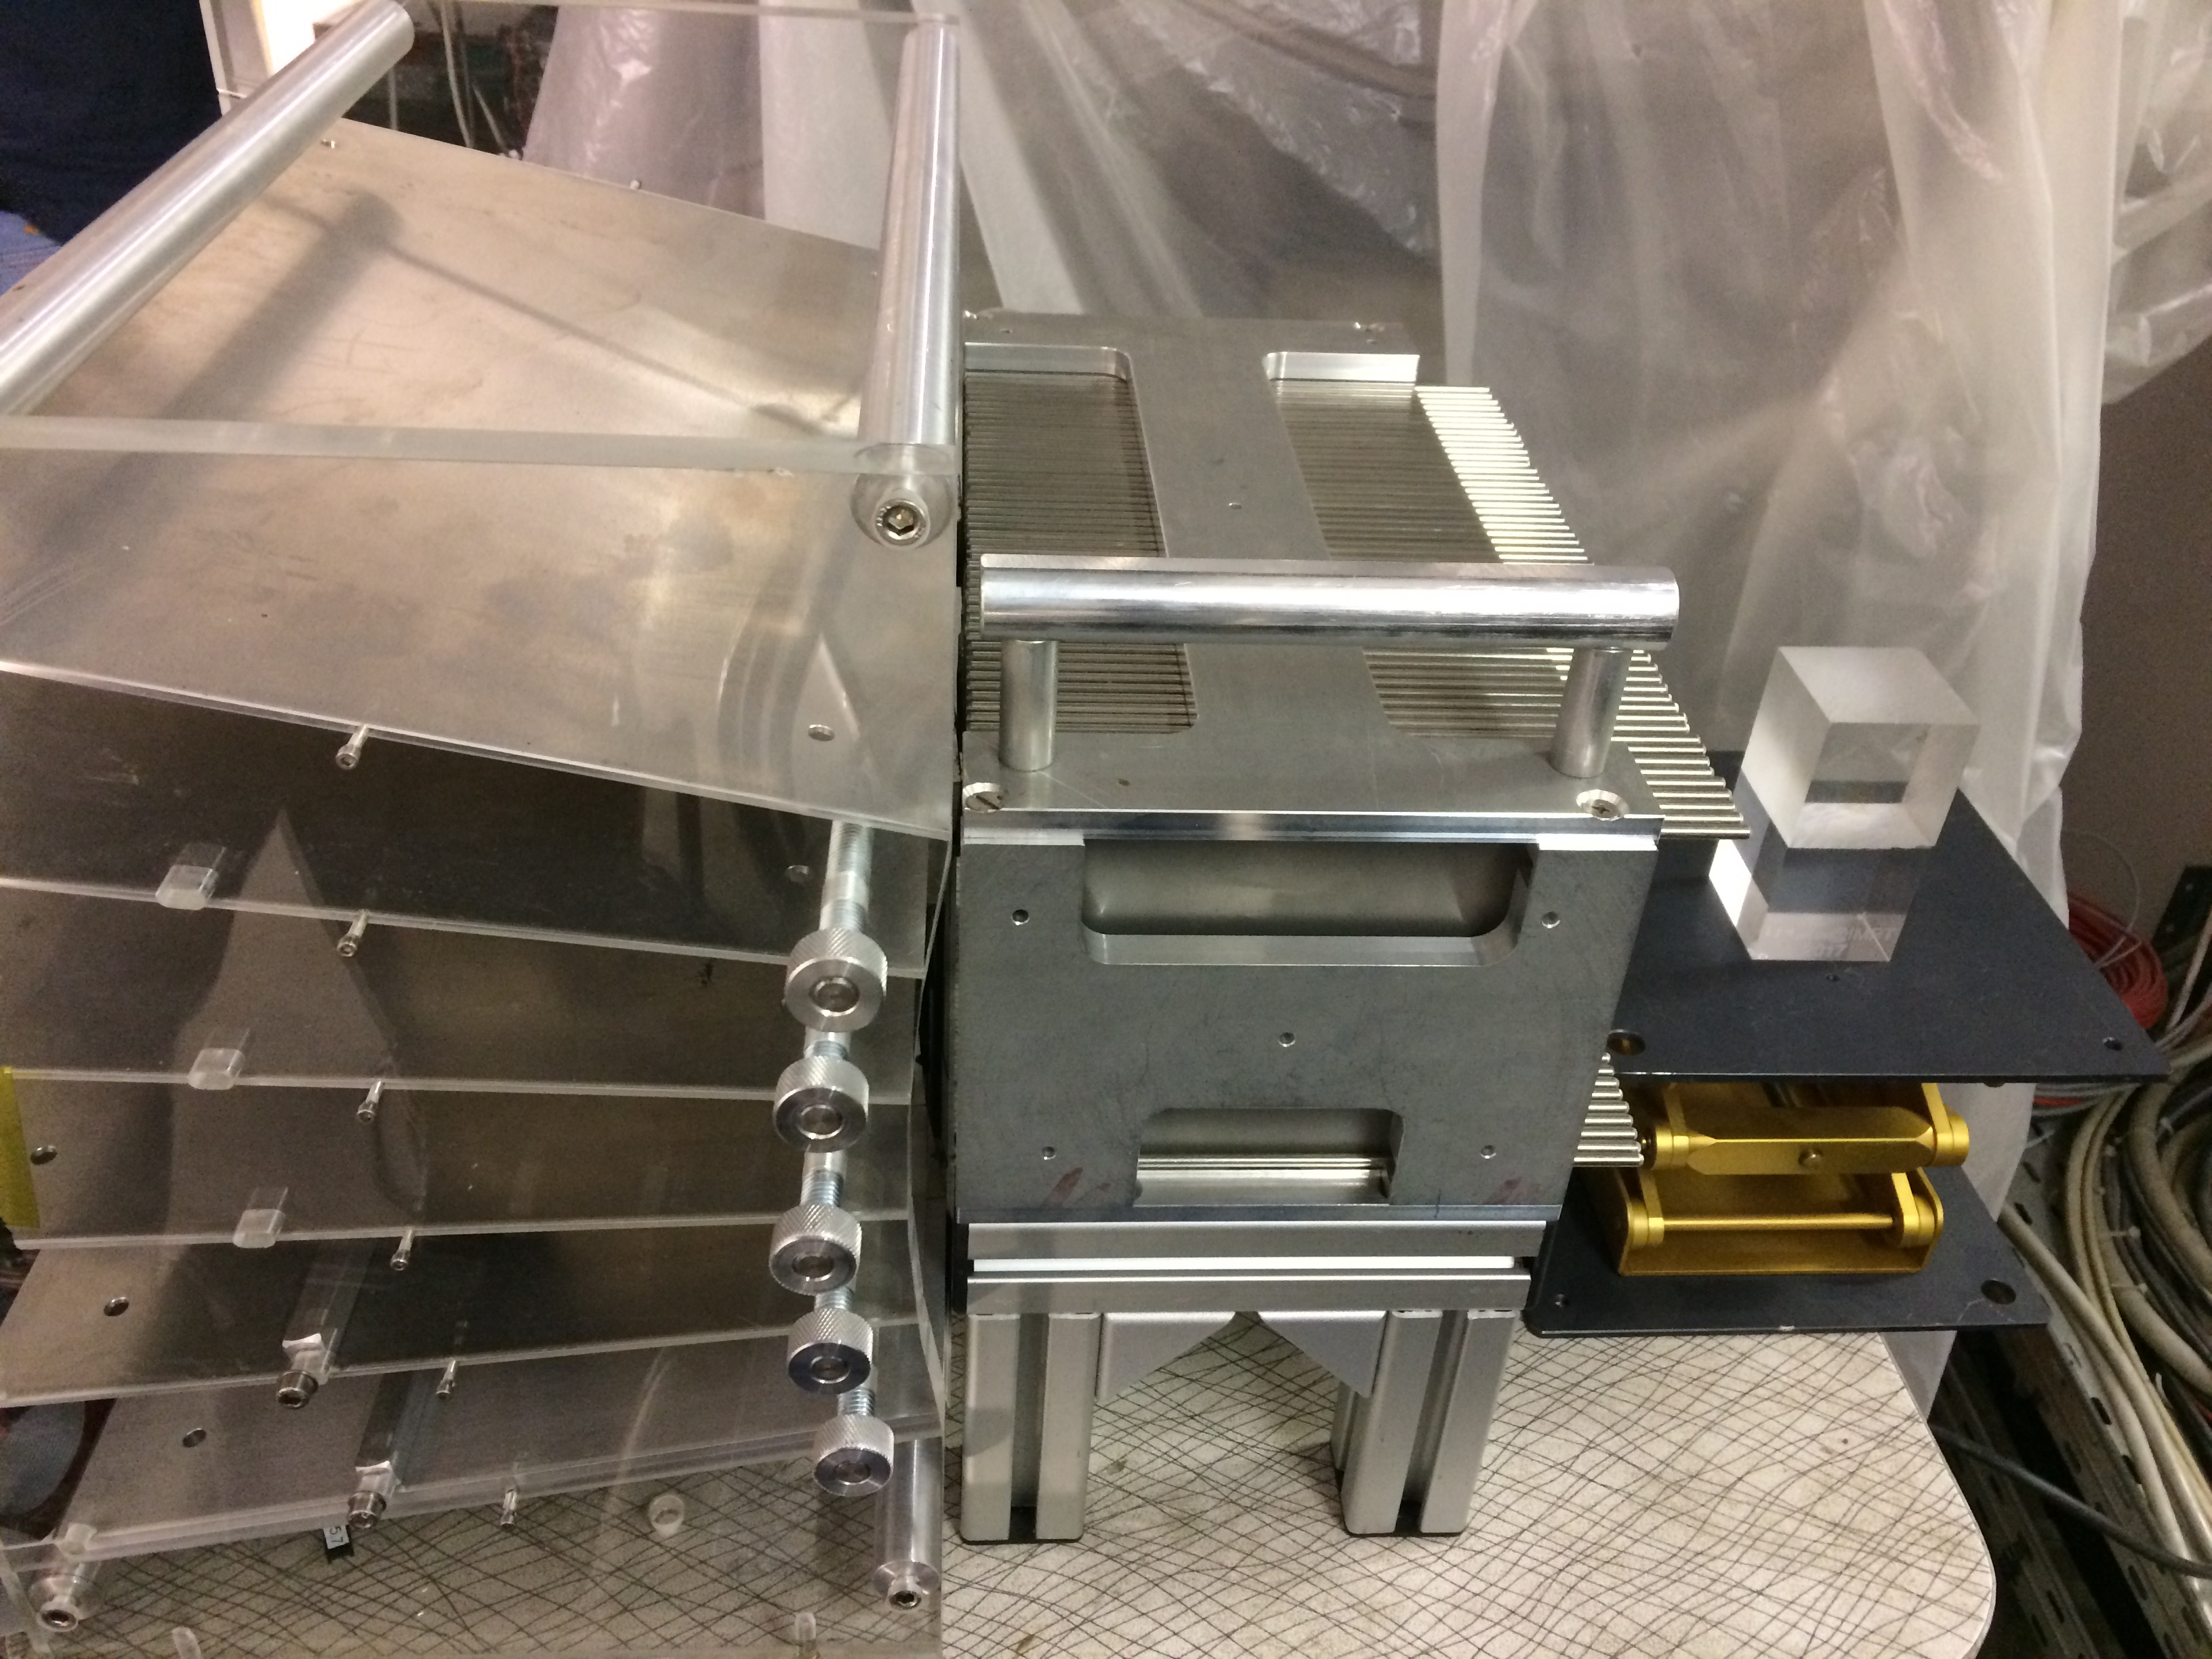
\includegraphics[width=1.\textwidth, height=5.5cm]{03_GraphicFiles/chapter6_BeamTests/Nice_September2018/Target_Coll_Abs_side.jpg}
\caption{Side view of the multi-collimated camera and \gls{pmma} target setup. The picture is taken from the nozzle side.}
\label{chap6::fig::September_SetupPicture}
\end{subfigure}
\begin{subfigure}[t]{.5\textwidth}
\centering
\includegraphics[width=1.\textwidth, trim = {0 20cm 0 30cm}, clip, height=5.5cm]{03_GraphicFiles/chapter6_BeamTests/Nice_September2018/Target_Coll_Abs_front.jpg}	
\caption{Front view of the multi-collimated camera and \gls{pmma} target setup. The beam direction is from left to right.}
\label{chap6::fig::September_SetupPicture2}
\end{subfigure}
\caption{Detailed views of the multi-collimated camera setup with the \gls{pmma} target cubes.}
\label{chap6::fig::September_SetupCameraDetails}
\end{figure}

The absorber has been initially tested in stand-alone acquisitions to first characterize the \gls{bgo} block response to beam-induced \glspl{pg}. Various runs have been performed with and without the collimator, with the target fixed in the initial position. For the irradiation without collimator, the distance between the target and the absorber blocks has been kept unchanged, and corresponded to 27~cm (10~cm distance target-collimator entrance face + 17~cm collimator thickness). The trigger rate was monitored online, as well as the detection rate of each single block. The power supply of each block has been adjusted with some low beam-intensity acquisitions without collimator to obtain compatible detection rate (in the range 300-400~kHz) on the 6 blocks. The beam current was approximately 150~pA. A set of measurements have been collected with this configuration. With the collimator, the beam current has been increased to obtain similar trigger rates, up to about 1~nA. In particular, two data sets have been collected with the collimator and with the target in two different positions: the initial one, and one shifted of 1~cm in the beam direction increasing the distance from the nozzle.
A second phase of the test has been dedicated to the synchronization of absorber and hodoscope, with the trigger to the hodoscope acquisition given by the absorber blocks (as in the final multi-collimated camera configuration). With the setup including the collimator and the target in the initial position, the beam intensity has been tuned in order to obtain a trigger rate of few kHz, corresponding to an hodoscope stand-alone detection rate of approximately 10~MHz, directly monitored by the hodoscope \gls{fe} board, as done in the May 2018 test described in section~\ref{chap6::sec::may2018}. Several data sets have been collected for different values of the coincidence window, and the \gls{tof} spectra have been produced.
The beam tests allowed to verify on beam the new developed features of the acquisition system, as well as to test for the first time the \gls{bgo} blocks with the final acquisition system, exposed to \glspl{pg}. The main results of the test are presented in the next section and discussed in section~\ref{chap6::subsec::septemberDiscussion}. 
   

\subsection{Experimental results}\label{chap6::subsec::septemberResults} 

\figurename~\ref{chap6::fig::september_rawNoCollimator} shows the data collected by the 6 \gls{bgo} absorber blocks without the collimator during the irradiation of the \gls{pmma} target, as visualized by the online monitoring tool mentioned in section~\ref{chap3::subsec::cameraSoftware}. The left side panels show, from top to bottom, the histogram of the number of hit blocks per events, the integrated distribution of the reconstructed interaction positions along the horizontal and vertical axes. The right panel shows the two-dimensional map of the reconstructed interaction position in the 6 blocks. The beam direction is from left to right in the presented plots. 
The \gls{pm} gain equalization step explained in section~\ref{chap3::subsec::absBGOchar} is already included in the monitoring code. The calibration factors for each \gls{bgo} block used in the beam test have been obtained during previous laboratory tests: the blocks have been exposed to a $^{22}$Na source and the data have been collected with the final acquisition system.  

\begin{figure}[!htbp]
\centering
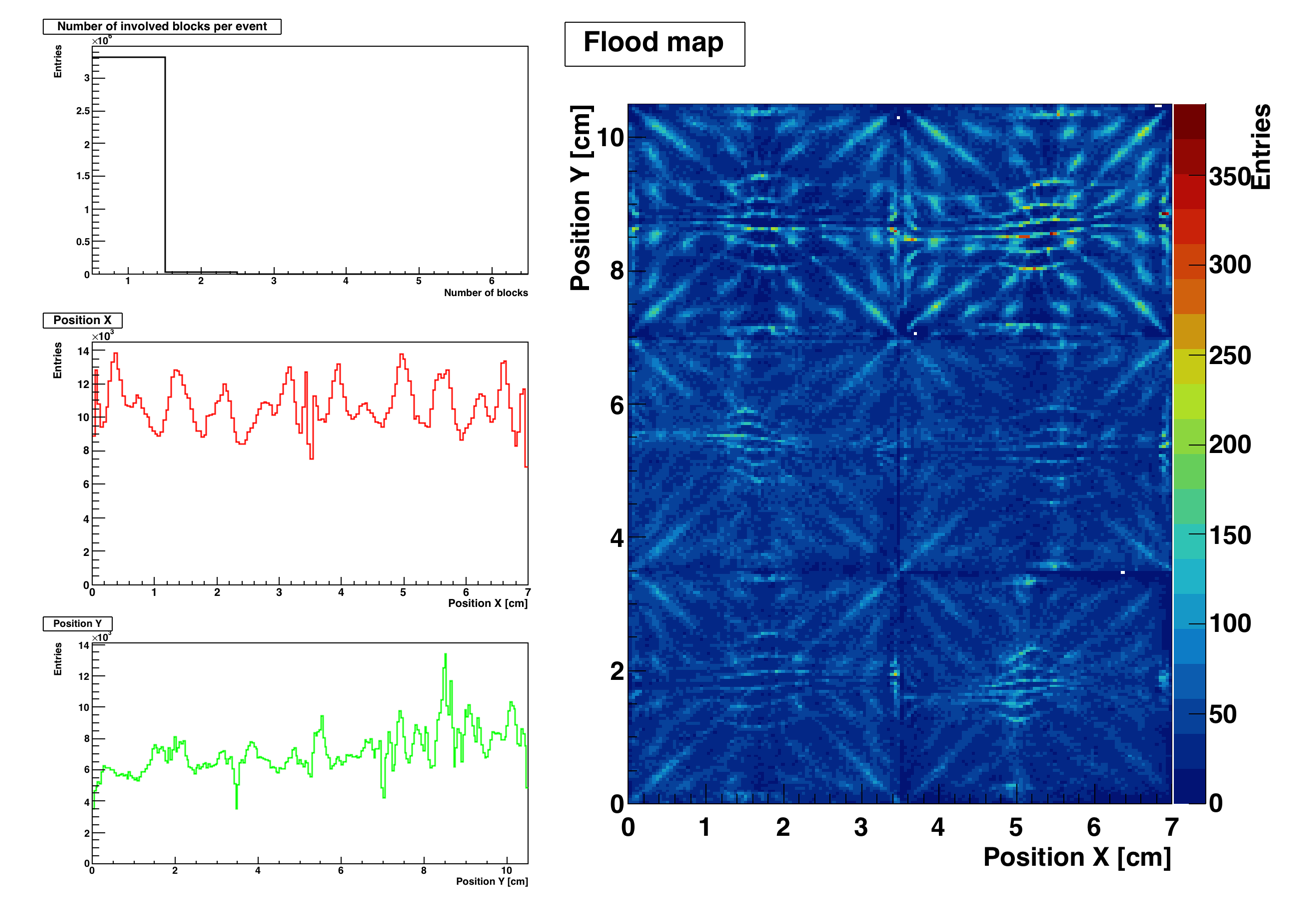
\includegraphics[width=0.9\textwidth]{03_GraphicFiles/chapter6_BeamTests/Nice_September2018/287_complete_NOcutAppl.png}
\caption{Raw data collected by the 6 absorber \gls{bgo} blocks during an irradiation of the \gls{pmma} without the collimator. On the left side, the top histogram show the number of blocks hit per event, the central and bottom histograms show the projection of the reconstructed interaction positions on the horizontal and vertical direction, respectively. The right side panel show the two-dimensional distribution of the reconstructed interaction positions. No data selection has been applied.}
\label{chap6::fig::september_rawNoCollimator}
\end{figure}

The data set collected without the collimator has been used to fine tune the analysis and calibration parameters (calibration factors, data selection). The results of the complete calibration and analysis processes are shown in the following for one of the employed blocks.

The effect of the \gls{pm} gain equalization are shown in \figurename~\ref{chap6::fig::absPM_amp}, where the signal integral spectra are presented for the four block \glspl{pm} before (left) and after (right) the gain equalization. In the right panel, the calibrated energy spectrum (sum of the four \gls{pm} signal integrals for each event) is also shown. 
The raw signals have been investigated to understand the origin of the peak in the spectra at the highest \gls{adc}/energy values (about 3200$\times$10$^3$ \gls{adc} counts - left plot- and about 5800~keV - right plot) and a significant amount of event presents signal amplitudes which are beyond the \gls{asm} board \gls{adc} saturation limit. Such events are rejected in the following analysis. 

\begin{figure}
\begin{subfigure}[t]{0.5\textwidth}
\centering
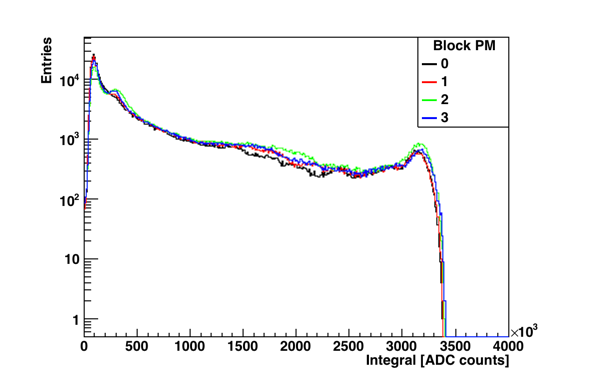
\includegraphics[width=1\textwidth]{03_GraphicFiles/chapter6_BeamTests/Nice_September2018/287_noSel/raw_PMhistos.png}
\caption{Before gain equalization.}
\label{chap6::fig::absPM_rawProfiles}
\end{subfigure}
\begin{subfigure}[t]{0.5\textwidth}
\centering
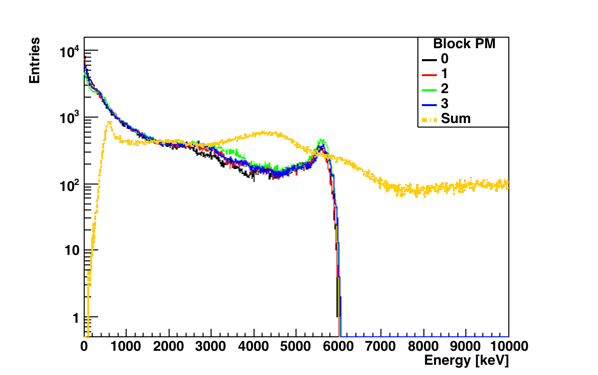
\includegraphics[width=1\textwidth]{03_GraphicFiles/chapter6_BeamTests/Nice_September2018/287_noSel/2_PM_canvas.png}
\caption{After gain equalization.}
\label{chap6::fig::absPM_calProfiles}
\end{subfigure}
\caption{\gls{pm} signal integral spectra.}
\label{chap6::fig::absPM_amp}
\end{figure}

The whole block energy spectra before (left) and after (right) the \gls{pm} gain equalization and event selection are sketched in \figurename~\ref{chap6::fig::absADCspectrum}. The processed spectrum shows the spectrospic gamma peaks expected for the irradiation of a \gls{pmma} target, corresponding to the de-excitation of $^{12}$C (4.44~MeV) and to the neutron capture by hydrogen (2.22~MeV - deuterium binding energy). In addition, the de-excitation of $^{16}$O {6.13~MeV} creates the spectrum slope change visible at about 6000~keV. The energy spectrum shows the contamination of background events below 1~MeV, which will be rejected in the following analysis.

\begin{figure} [!h]
\begin{subfigure}[t]{0.5\textwidth}
\centering
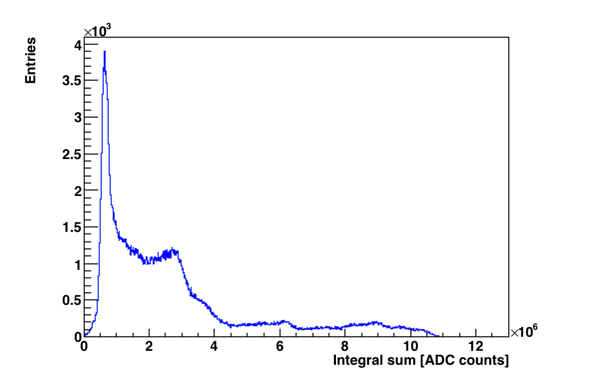
\includegraphics[width=1\textwidth]{03_GraphicFiles/chapter6_BeamTests/Nice_September2018/287_noSel/raw_Espectrum.png}
\caption{Before gain equalization and saturated events rejection.}
\label{chap6::fig::absRaw_Espectrum}
\end{subfigure}
\begin{subfigure}[t]{0.5\textwidth}
\centering
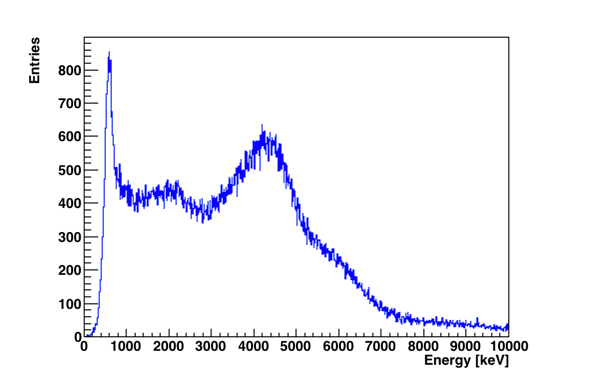
\includegraphics[width=1\textwidth]{03_GraphicFiles/chapter6_BeamTests/Nice_September2018/287_noSel/2_Espectrum_canvas_cal.png}
\caption{After gain equalization and saturated events rejection.}
\label{chap6::fig::absCal_Espectrum}
\end{subfigure}
\caption{Whole block energy spectrum.}
\label{chap6::fig::absADCspectrum}
\end{figure}

The mono-dimensional integrated profiles and the two-dimensional maps of the reconstructed interaction positions are shown in \figurename~\ref{chap6::fig::absXYprofiles} and \figurename~\ref{chap6::fig::absFloodMap}, respectively, before (left) and after (right) the calibration and energy selection processes. 

\begin{figure}
\begin{subfigure}[t]{0.5\textwidth}
\centering
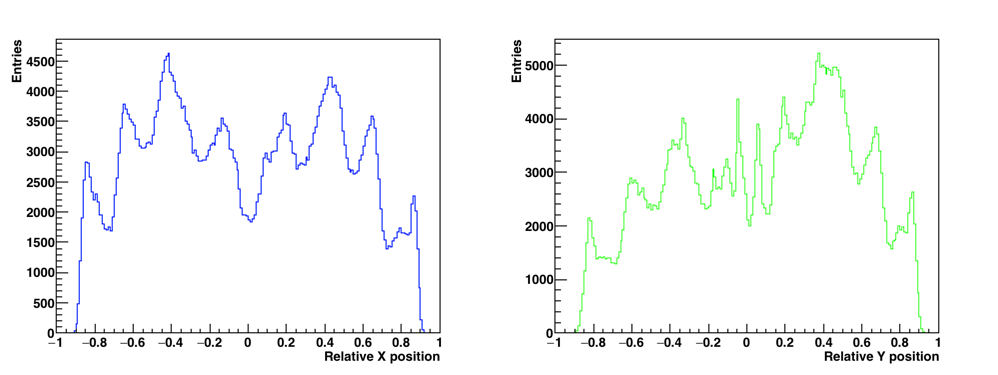
\includegraphics[width=1.05\textwidth]{03_GraphicFiles/chapter6_BeamTests/Nice_September2018/287_noSel/raw_1dProfiles.png}
\caption{Before gain equalization, saturated events rejection, and event energy selection.}
\label{chap6::fig::abssingleAxisRawProfile}
\end{subfigure}
\begin{subfigure}[t]{0.5\textwidth}
\centering
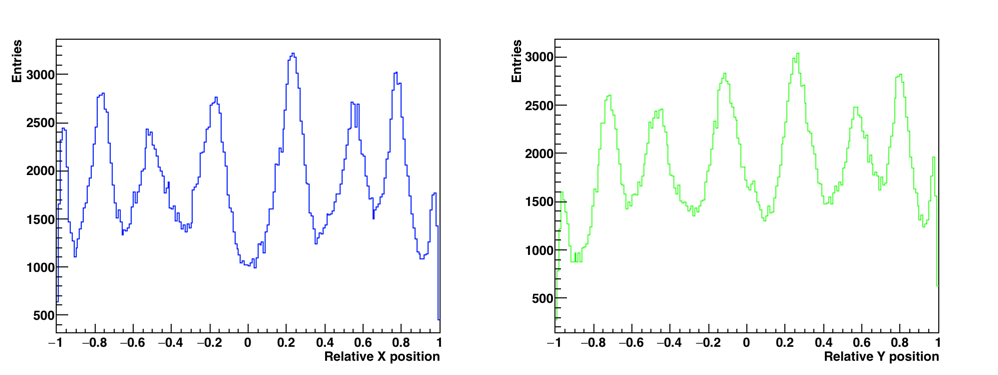
\includegraphics[width=1.05\textwidth]{03_GraphicFiles/chapter6_BeamTests/Nice_September2018/287_noSel/2_profile_canvas_cal.png}
\caption{After gain equalization, saturated events rejection, and event energy selection.}
\label{chap6::fig::abssingleAxisCalProfile}
\end{subfigure}
\caption{1D integrated position distribution on the two transverse dimensions. In the two sub-figures, left side for the horizontal dimension (x), right side for the vertical one (y).}
\label{chap6::fig::absXYprofiles}
\end{figure}

\begin{figure} [!h]
\begin{subfigure}[t]{0.5\textwidth}
\centering
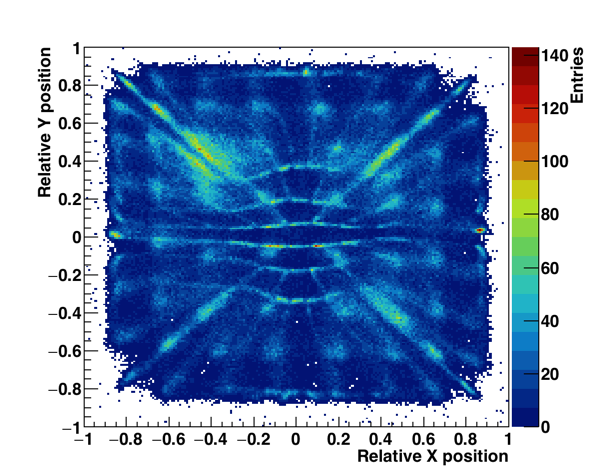
\includegraphics[width=1\textwidth]{03_GraphicFiles//chapter6_BeamTests/Nice_September2018/287_noSel/raw_2dMap.png}
\caption{Before gain equalization, saturated events rejection, and event energy selection..}
\label{chap6::fig::absraw_floodMap}
\end{subfigure}
\begin{subfigure}[t]{0.5\textwidth}
\centering
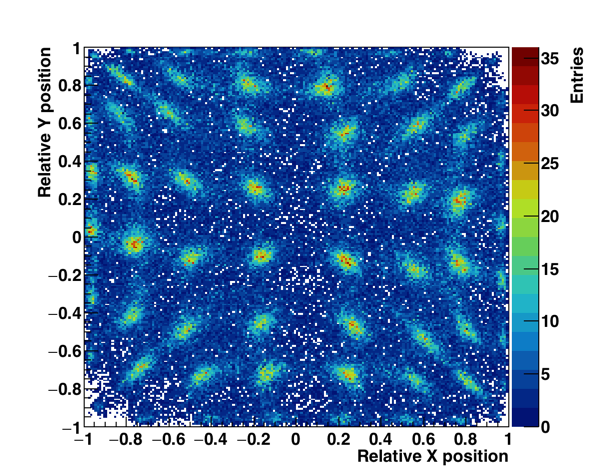
\includegraphics[width=1\textwidth]{03_GraphicFiles//chapter6_BeamTests/Nice_September2018/287_noSel/2_flood_canvas.png}
\caption{After gain equalization, saturated events rejection, and event energy selection.}
\label{chap6::fig::abscal_floodMap}
\end{subfigure}
\caption{2D maps of the reconstructed interaction positions.}
\label{chap6::fig::absFloodMap}
\end{figure}

The described analysis steps have been applied to the data collected by the 6 blocks, and the resulting distributions are shown in \figurename~\ref{chap6::fig::september_selNoCollimator}, to be compared to \figurename~\ref{chap6::fig::september_rawNoCollimator}.
\begin{figure}[!htbp]
\centering
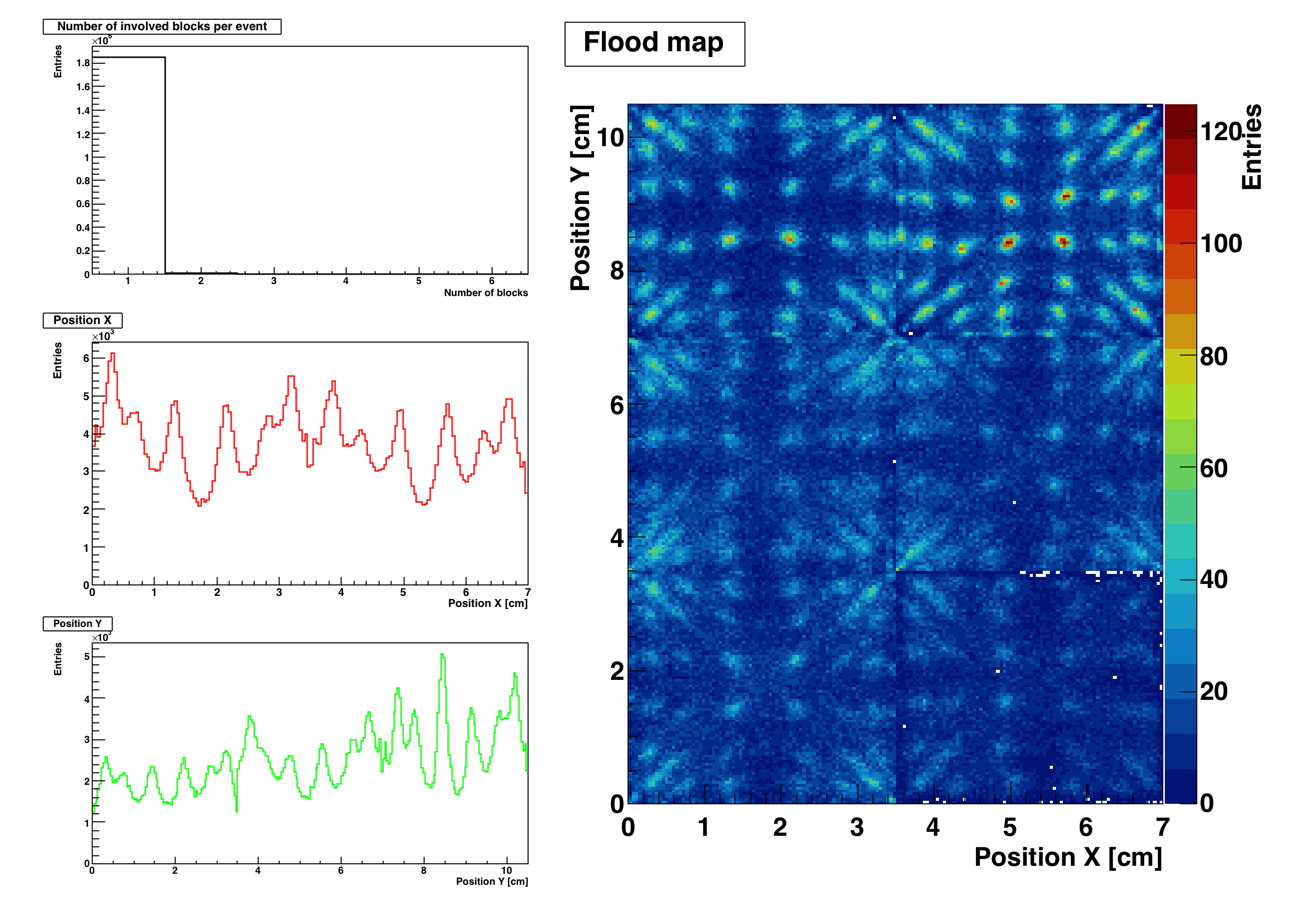
\includegraphics[width=0.9\textwidth]{03_GraphicFiles/chapter6_BeamTests/Nice_September2018/287_complete_cutAppl.png}
\caption{As for \figurename~\ref{chap6::fig::september_rawNoCollimator}, with the selection of events below the \gls{asm} board \gls{adc} saturation limit and with an deposited energy higher than 1~MeV.}
\label{chap6::fig::september_selNoCollimator}
\end{figure}

Once properly calibrated and selected, the data obtained with the acquisition without collimator have been used to extract efficiency calibration factors to be used for the analysis of the data collected during irradiation with the collimator. As shown in section~\ref{chap3::subsec::absBGOchar}, indeed, the detection efficiency significantly varies on the surface of each block, so that the collected data must be normalized according to the interaction position on the block surface. To be noticed that such an efficiency dis-uniformity is expected to be reduced at increasing gamma incident energy, but the blocks had not been exposed to gamma energies above 1.3~MeV before this beam test. The interaction position profile must be reconstructed along the beam direction (x), so that the normalization factors are extracted by the mono-dimensional x position profile (see \figurename~\ref{chap6::fig::abssingleAxisCalProfile} - left). 

The mono-dimensional interaction position profile along the beam direction for two acquisition with a target relative shift of 1~cm is shown in \figurename~\ref{chap6::fig::september_profiles}. The two profiles have been normalized to their maximum. The bin size has been chosen to represent half of the \gls{bgo} block pseudo-pixel size.

\begin{figure}[!htbp]
\centering
\hspace{-1.5cm} 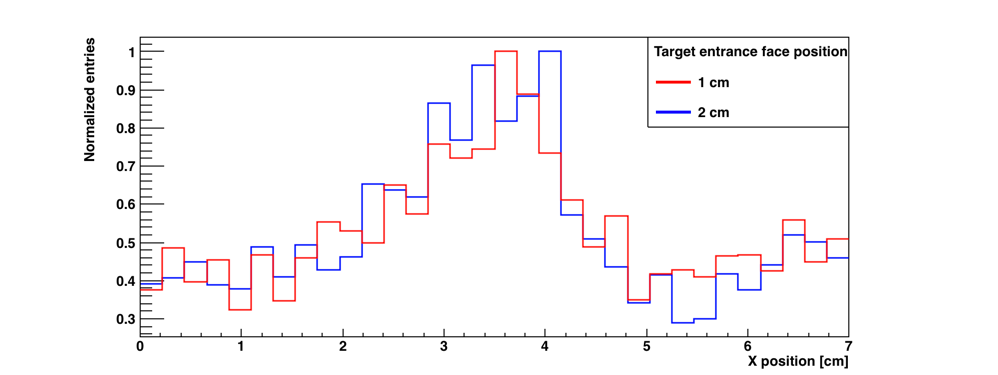
\includegraphics[width=1.1\textwidth]{03_GraphicFiles/chapter6_BeamTests/Nice_September2018/profile_compl.png}
\caption{Mono-dimensional interaction position profile along the beam direction obtained for two acquisitions with the \gls{pmma} target set in two different positions. The red curve corresponds to the run with the target entrance face at 1~cm from the absorber block entrance face in the beam direction, while the blue curve corresponds to a 1~cm shift in the beam direction, so with the target entrance face at 2~cm from the absorber block entrance face.}
\label{chap6::fig::september_profiles}
\end{figure}

The two distribution peaks correspond to the expected proton range in the \gls{pmma} target, which is approximately 2.5~cm considering the residual proton range after the interaction in the hodoscope. A shift in such peaks for the two target positions is visible and estimated in 6~mm. 

As mentioned, in the second part of the beam test the synchronization and timing performance of the coupling of hodoscope and multi-collimated camera have been tested. In \figurename~\ref{chap6::fig::september_TOF} the \gls{tof} spectrum obtained with a 120~ns coincidence window is shown. The \gls{tof} is here defined as the difference between the trigger time and the arrival time of the first interaction recorded in the hodscope, and the coincidence window starts at the trigger arrival time, with the coincidence research performed in the time window preceding the trigger.

\begin{figure}[!htbp]
\centering
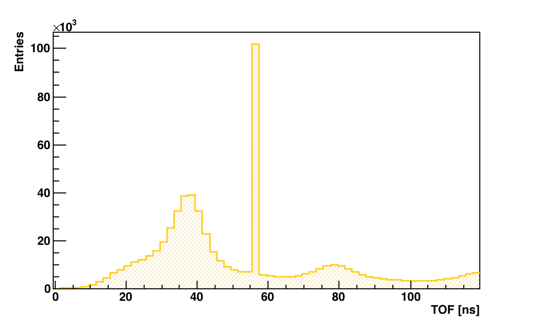
\includegraphics[width=0.8\textwidth]{03_GraphicFiles/chapter6_BeamTests/Nice_September2018/TOF_0-120ns_rev_fill_lessBins.png}
\caption{\gls{tof} spectrum obtained with hodoscope and multi-collimated camera with a coincidence window of 120~ns.}
\label{chap6::fig::september_TOF}
\end{figure}

The \gls{tof} distributions shows the beam time structure, with bunches delivered each 20~ns. Two bunches are clearly visible in the presented distribution, and a third one is cut by the end of the coincidence window. The peak at the center of the distribution is caused by a problem in the 250~ps resolution clock value conversion in the hodoscope \gls{fe} board, discussed in section~\ref{chap6::subsec::septemberDiscussion}.  

\subsection{Discussion}\label{chap6::subsec::septemberDiscussion} 

A minimal multi-collimated camera configuration, composed of 6 \gls{bgo} blocks and the tungsten collimator described in chapter~\ref{chap::3}, has been tested on beam with the final \gls{utca}-based acquisition system for the first time. In addition to this, the coupling between absorber and hodoscope has been tested for \gls{tof} measurements. 
The test provided encouraging outcomes: it allowed to obtain a first estimate of the camera performance, even if in a non-optimized version, and to plan the further development needed. 
In particular, \figurename~\ref{chap6::fig::september_profiles} shows the potential of the camera in detecting range shifts in a homogeneous target. For a 1~cm target shift, a 6~mm shift is detected in the peak of the mono-dimensional interaction position profiles. For this test, the 6 employed blocks have been vertically aligned, but different solutions will be studied in future laboratory and beam tests to improve the spatial resolution by relatively shifting the block pseudo-pixel positions in a column. Moreover, the collimator multi-slit width can be varied to asses the best configuration according to the block spatial resolution. 
The retrieved performance are determined by the block calibration process developed with a preliminary acquisition system (see section~\ref{chap3::subsec::absBGOchar}) and for the first time adapted to the final acquisition logic, based on raw signal integrals. 
It must be noticed that the pixel-based energy calibration could not be performed due to the limited statistics. Extensive laboratory tests with the \gls{utca} acquisition system, foreseen in the next months, will allow to optimize the block calibration process, and a performance improvement is expected. Moreover, the block and \gls{asm} card working parameters will be further studied to reduce the amount of events saturating the \gls{adc} limits. However, overall better performance have been verified with a signal amplification stage preceding the conversion to logic (as done with the preliminary acquisition system), so that the development of new \gls{fe} cards including a shaping amplifier dedicated to each block \gls{pm} can in principle significantly improve the detector performance. The proposed solutions will be evaluated in the next future and new tests focused on the absorber detector are already planned before the end of 2018. 
Concerning the \gls{tof} measurements, the beam time structure could be clearly identified, and a data \gls{tof} selection will be tested in next beam measurements. Improvements in the hodoscope \gls{fe} board firmware, already discussed in section~\ref{chap6::subsec::mayDiscussion}, are expected to improve the coincidence time resolution, which will be also enhanced with the aforementioned optimization of the absorber block response. In particular, the shaping-amplification stage proposed for the \gls{bgo} block raw signal would in principle allow for more accurate time measurements. Finally, the time conversion artifacts highlighted in the comments to \figurename~\ref{chap6::fig::september_TOF} have been identified and will be corrected in a new version of the hodoscope \gls{fe} card firmware developed by the \gls{ipnl} electronics group.
The camera performance obtained during this tests are still not satisfactory if considering the design expectations and the monitoring objectives, but all the proposed system improvements are expected to enhance the camera spatial and time response. As mentioned, new beam tests are already planned for the next months: a first test will be dedicated to a detailed characterization of the available set of \gls{bgo} blocks on beam and to fine tune the blocks and \gls{asm} board working parameters, as well as to optimize the collimator geometrical configuration.
  


\clearpage
%\printbibliography[heading=subbibintoc]
